
%%% Local Variables:
%%% mode: latex
%%% TeX-master: ".."
%%% End:

\section{grid绘图系统}
\begin{frame}{\subsecname}{}
  % \begin{columns}
  %   \begin{column}{.\textwidth}
  %     \begin{figure}
  %       \centering 
\includegraphics[width=\columnwidth]{桃花源记.png}
  %     \end{figure}
  %   \end{column}

  %   \begin{column}{.5\textwidth}
  %     \begin{ornamentblock}
  %       { 林尽水源,便得一山,山有小口,仿佛若有光。便舍船,从口入。初极狭,才通人。复行数十步,豁然开朗。土地平旷,屋舍俨然,有良田美池桑竹之属。阡陌交通,鸡犬相闻。其中往来种作,男女衣着,悉如外人。黄发垂髫,并怡然自乐。\\
  %         \rightline{\textemdash《陶渊明·桃花源记》}}
  %     \end{ornamentblock}
  %   \end{column}
  % \end{columns}
  \begin{minipage}{\textwidth}
      \begin{ornamentblock}
        { 林尽水源,便得一山,山有小口,仿佛若有光。便舍船,从口入。初极狭,才通人。复行数十步,豁然开朗。土地平旷,屋舍俨然,有良田美池桑竹之属。阡陌交通,鸡犬相闻。其中往来种作,男女衣着,悉如外人。黄发垂髫,并怡然自乐。\\
          \rightline{\textemdash《陶渊明·桃花源记》}}
      \end{ornamentblock}
  \end{minipage}
  \begin{minipage}{\textwidth}
     \centering 
\includegraphics[width=0.6\columnwidth]{桃花源记.png}
  \end{minipage}
\end{frame}

\subsection{来龙去脉}
\begin{frame}[t,fragile]{\subsecname}{}
\begin{itemize}
\item<1-> 前面介绍的graphics程序包是R的标准绘图系统,也称为\emphText{graphics绘图系统},
  除此之外R中还有另一套截然不同的\emphText{grid绘图系统}
\item<1-> 使用grid绘图系统前需要先用\emphText{library(grid)}加载grid程序包,
该程序包由\href{https://www.stat.auckland.ac.nz/~paul/}{\uline{Paul Murrell}}开发维护
%\textsuperscript{\underline{\href{https://www.stat.auckland.ac.nz/~paul/}{主页}}} 
\item<2-> grid绘图系统的\emphText{设计初衷是为了克服graphics系统中元素不能动态修改的弱点}
\end{itemize}

\vspace{-10pt}
\begin{overlayarea}{\textwidth}{\textheight}
\only<1>{
\begin{figure}\centering
  \captionsetup[subfigure]{labelformat=empty} 
  \subfloat[]
  {
\includegraphics[height=0.4\textheight]{paul_murrell.jpg}} \vspace{1pt}
  \subfloat[]
  {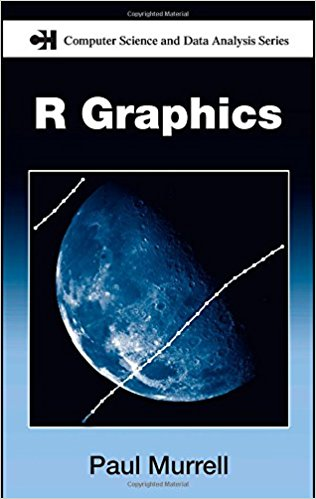
\includegraphics[height=0.4\textheight]{R_graphics_cover.jpg}} \vspace{-10pt}
  \caption{左图是grid作者Paul Murrell,目前是奥克兰大学统计系副教授;右图是他在2005年写的
书—《R Graphics》,现在已成为R领域的经典入门书籍}  
\end{figure}}

\only<3>{
\begin{block}{\small grid系统和graphics系统的区别} \footnotesize
\begin{itemize} 
\item[\HandRight] grid用\emphText{视口(viewports)}将绘图设备分割为不同的区域,
绘图对象(grob)可以在不同的视口中进行共享,比graphics中的处理方式更加灵活
\item[\HandRight] grid绘图对象可以被修改或者从一个图形中移除,\emphText{而不需要重新绘制所有的图形},
但是在graphics中则必须重绘 
\item[\HandRight] grid绘图系统是一个绘图框架,其原生的grid程序包仅提供低级绘图函数用于绘制统计图形中的元素,
不像graphis程序包还集成了高级绘图函数用于绘制常用的统计图形,
因此\emphText{直接用grid程序包绘制统计图形比较繁琐}
\item[\HandRight] \emphText{两套系统的绘图函数和绘图参数完全不同,不能混用!}
\end{itemize}
\end{block}}

\begin{onlyenv}<2>
\begin{columns}
  \begin{column}[t]{.5\textwidth}
    \begin{rcode}
# 基础统计图形库处理方式
plot(0:1, 0:1)
rect(0, 0, 1, 1, col = "red")
# 为了改变颜色,必须重画整幅图形
plot(0:1, 0:1)
# 虽然可以用新的矩形覆盖旧的,但旧矩形仍然存在
rect(0, 0, 1, 1, col = "blue")
    \end{rcode} 
  \end{column}

  \begin{column}[t]{.5\textwidth}
    \begin{rcode}
# grid绘图系统的处理方式
grid.rect(name = "rect0")
# 修改它的填充颜色为红色
grid.edit("rect0", gp = gpar(fill = "red"))
# 修改为蓝色,不需要重新用grid.rect()画矩形
grid.edit("rect0", gp = gpar(fill = "blue"))
    \end{rcode} 
  \end{column}
\end{columns} 
\end{onlyenv}

\only<4>{
\begin{figure}[t]
\centering
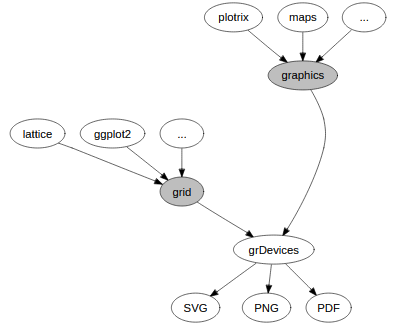
\includegraphics[width=0.45\columnwidth]{grid_system.png}
\caption{\emphText{lattice}和\emphText{ggplot2}是基于grid包开发的绘图程序包,这样就在grid
绘图系统中使用高级绘图函数来简化统计图形的绘制过程}
\end{figure}}
\end{overlayarea}
\end{frame} 

\subsection{lattice程序包}
\begin{frame}[t,fragile]{\subsecname}{}
\begin{itemize}
\item lattice程序包是基于grid包的编写的一套统计图形库,2000年发布了第一个版本,由
\href{https://www.isid.ac.in/~deepayan/}{\uline{Deepayan Sarkar}}等人开发维护,从R 3.0版本开始纳入base包,\emphText{不需要再单独安装}
\item lattice设计理念来自S-PLUS中的Trellis图形,是一种\emphText{多元数据可
视化的方法}:首先将多元数据分类组织,然后将绘图元素都 保存在一个\emphText{trellis对象}中,最后在\emphText{嵌板(panel)}区域绘制该对象,并且在panel上方用
\emphText{条板(strip)}区域来描述分类信息
\end{itemize}

\vspace{-8pt}
\begin{overlayarea}{\textwidth}{\textheight}
\only<1>{
\begin{figure}[ht]
  \centering
  
\includegraphics[width=0.7\columnwidth]{deepayan_sarkar.png}
  \caption{lattice程序包作者Deepayan Sarkar,目前是印度统计研究院的研究员}
\end{figure}}

\only<2>{
\begin{figure}[ht]
  \centering
  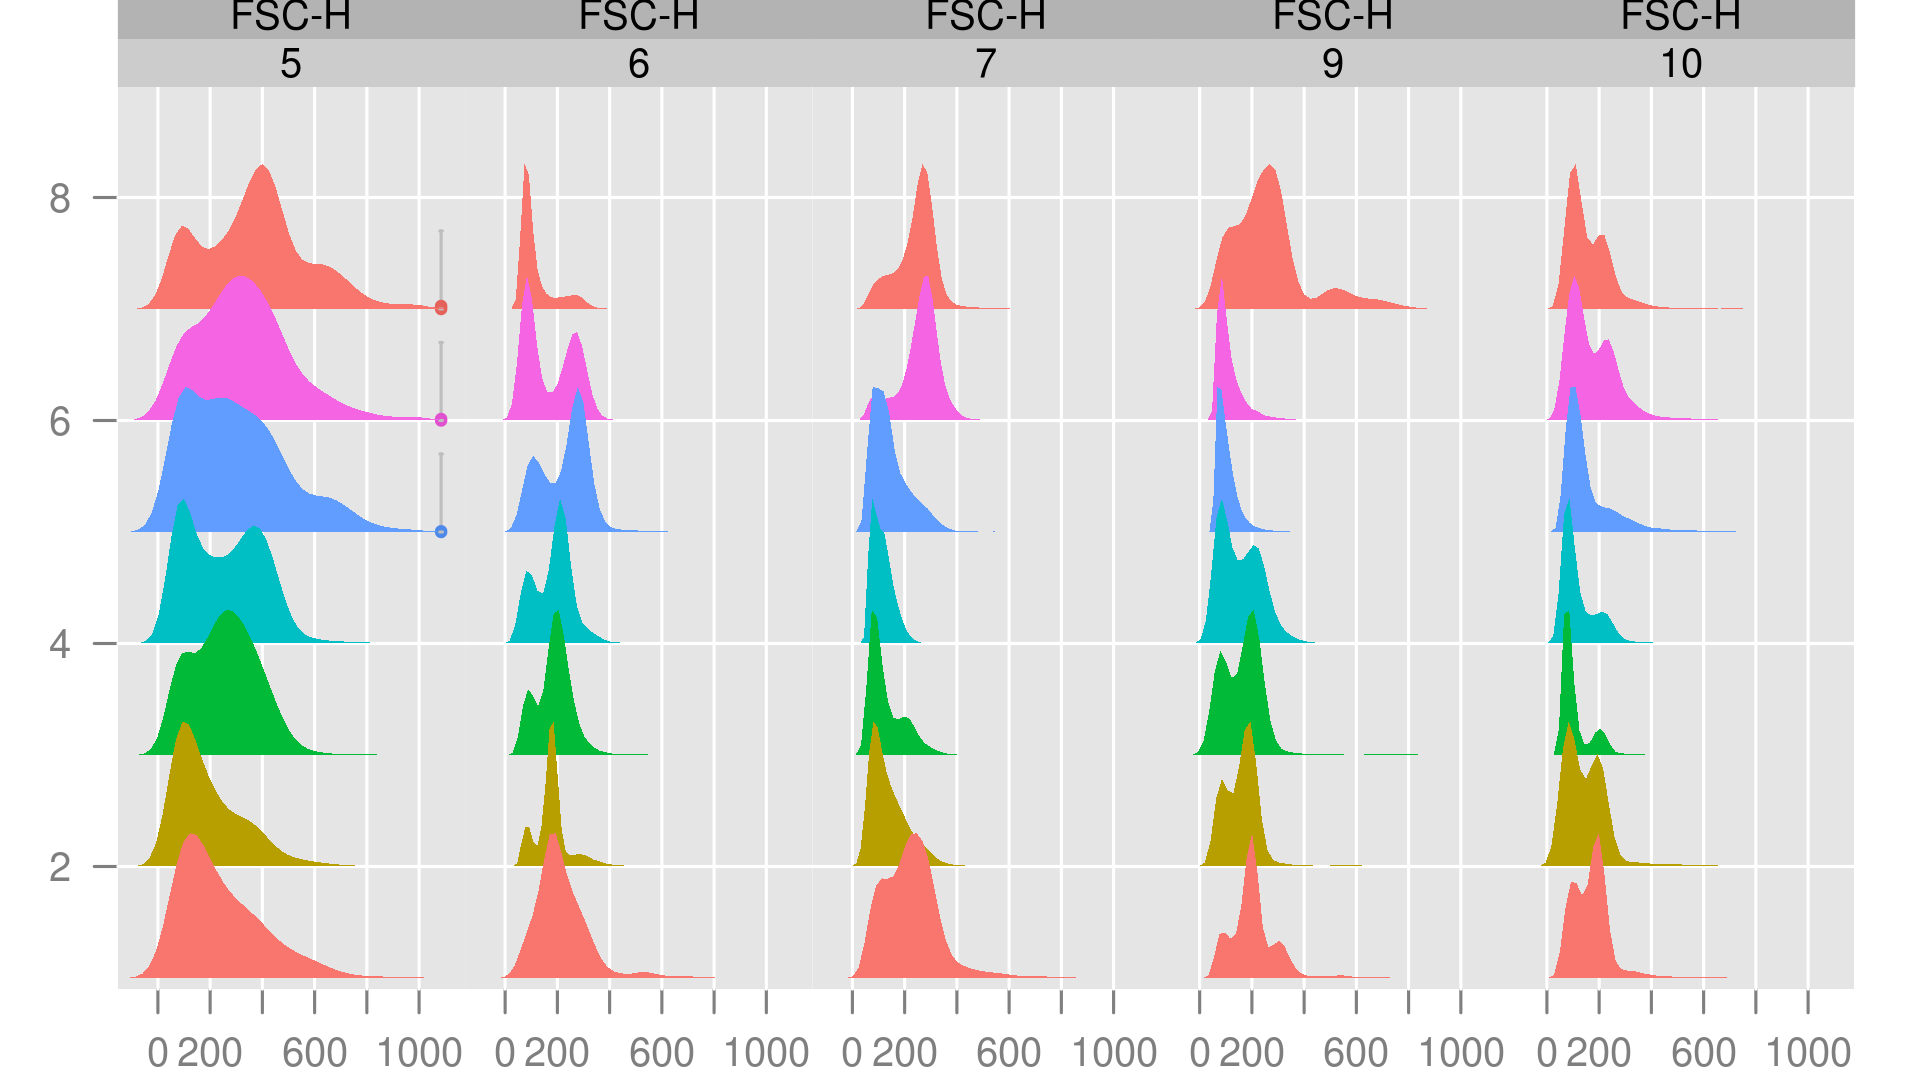
\includegraphics[width=0.7\columnwidth]{lattice-example1.png}
  \caption{不同的GvHD病患者在细胞检测中的FSC-H结果数据}
\end{figure}}

\only<3>{
\begin{figure}[ht]
  \centering
  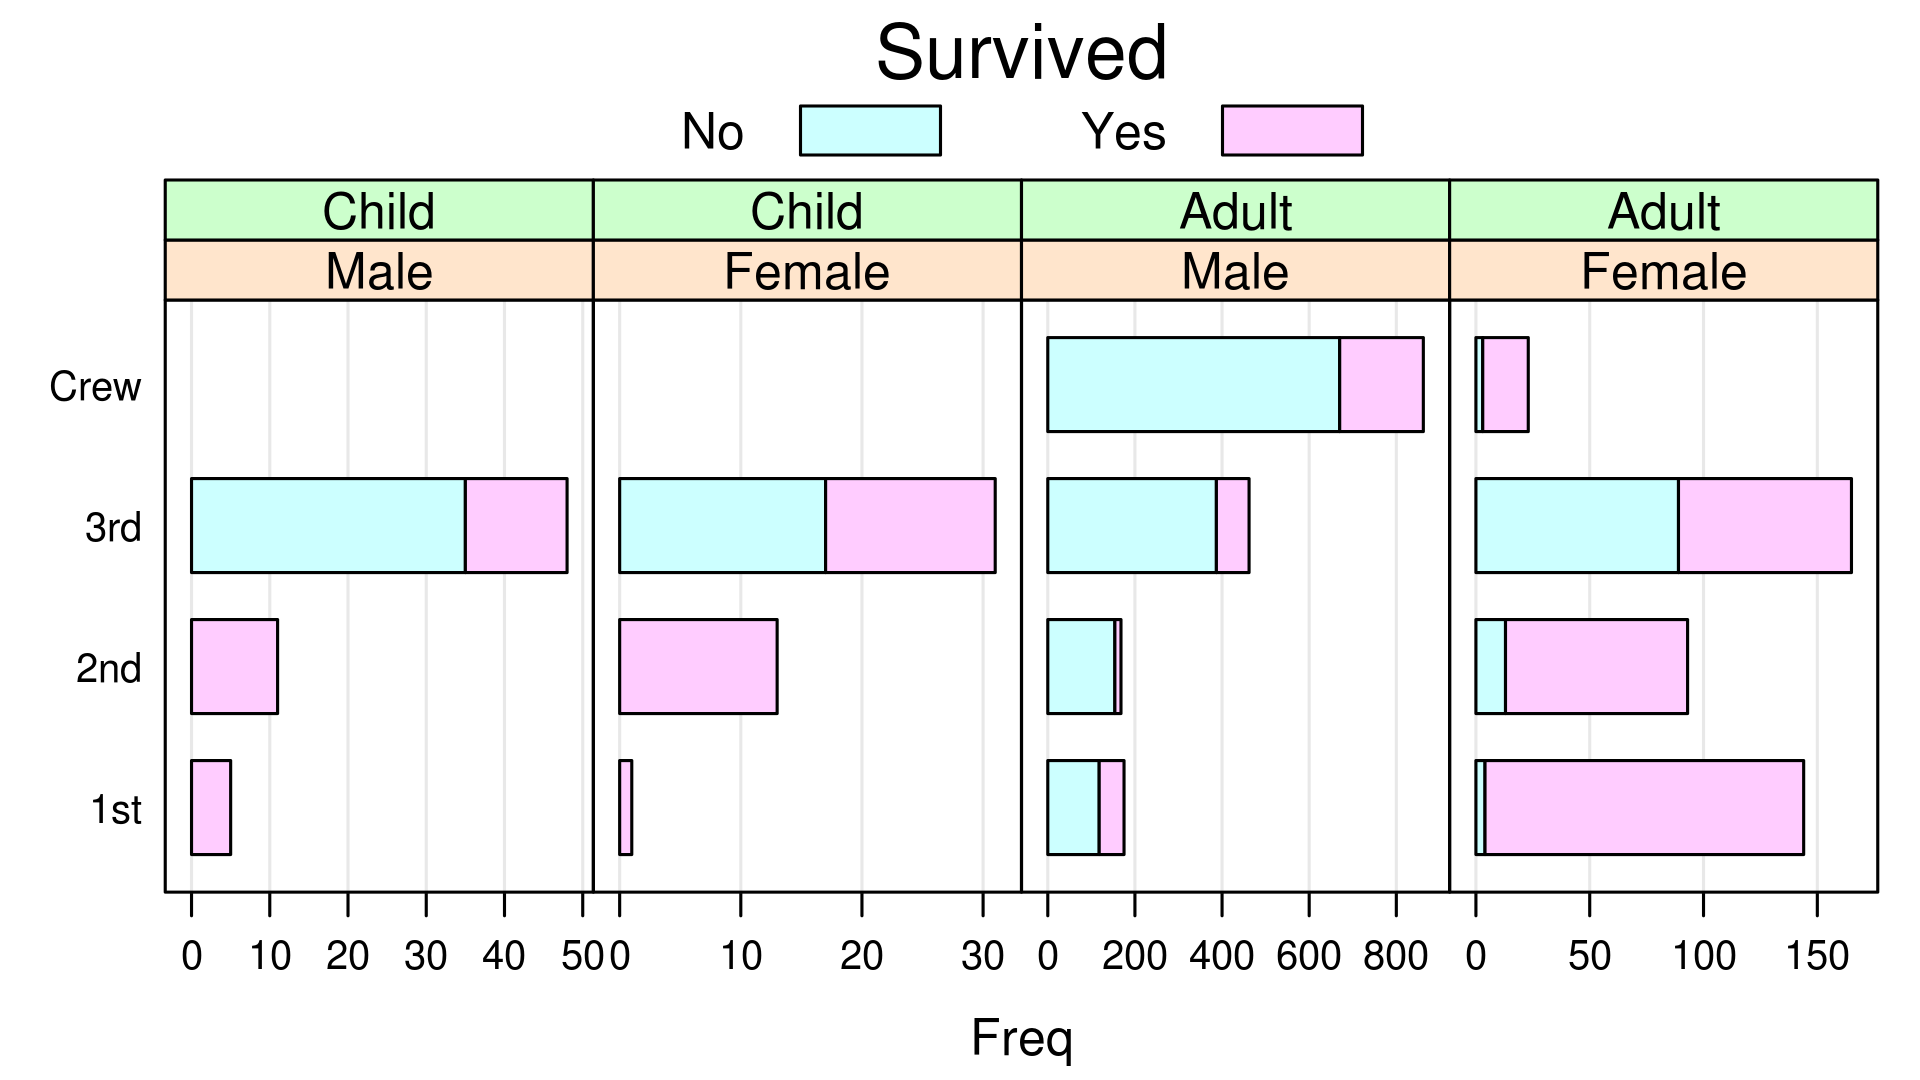
\includegraphics[width=0.7\columnwidth]{lattice-example2.png}
  \caption{泰坦尼克号生存率的交叉分类数据}
\end{figure}}
\end{overlayarea}  
\end{frame} 

\begin{frame}[t]{\subsecname}{公式参数}
\begin{itemize}
\item lattice的绘图函数都会\emphText{用公式作为第一位置参数}
\item<2-> 如果在不同panel中绘制多元数据,公式参数根据\emphText{“|”}符号后的变量对数据进行分类
\item<3-> 如果是在同一panel中绘制多元数据,则使用\emphText{group参数}对数据进行分类
\end{itemize}

\begin{overlayarea}{\textwidth}{\textheight}
\only<2>{
  \begin{table} \centering \footnotesize
    \begin{tabular}{|>{\centering\arraybackslash} m{0.2\columnwidth}|m{0.7\columnwidth}|}
      \toprule
      \rowcolor{LightCyan}
      \multicolumn{1}{|c|}{\textbf{公式参数}} & \multicolumn{1}{c|}{\textbf{含义}} \\\hline
      $\sim y$ & 单变量数据\\\hline
      $\sim y|z$ & 根据z变量对单变量数据划分panel\\\hline
      $y\sim x$ & 二元变量数据\\\hline
      $y\sim x|z $ & 根据z变量对二元变量数据划分panel\\\hline
      $y\sim x|a+b$ & 根据多条件变量划分panel,等价于$y\sim x|a$和$y\sim x|b$ \\\hline
      $y_1+y_2\sim x$ & 多元变量数据绘图,等价于$y_1\sim x$,和$y_2\sim x$\\\hline
      $z\sim x*y$ & 绘制三维图形(x,y,z)\\
      \bottomrule
    \end{tabular}
    \caption{lattice中的公式参数}
  \end{table}}
\end{overlayarea}
\end{frame} 

\begin{frame}[t,fragile]{\subsecname}{公式参数}
\begin{onlyenv}<1>
\begin{rcode}
> densityplot(|\colorbox{green}{$\sim$mpg}|, data=mtcars)
\end{rcode}
\begin{figure}
  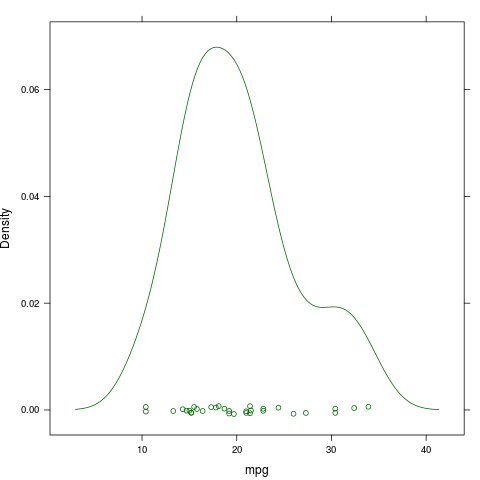
\includegraphics[width=0.6\columnwidth]{lattice-parameter1.png}
  \caption{在panel中绘制单变量数据}
\end{figure}
\end{onlyenv}

\begin{onlyenv}<2>
\begin{rcode}
> densityplot(|\colorbox{green}{$\sim$mpg\textbar cyl}|, data=mtcars, layout=c(1,3))
\end{rcode}
\begin{figure}
  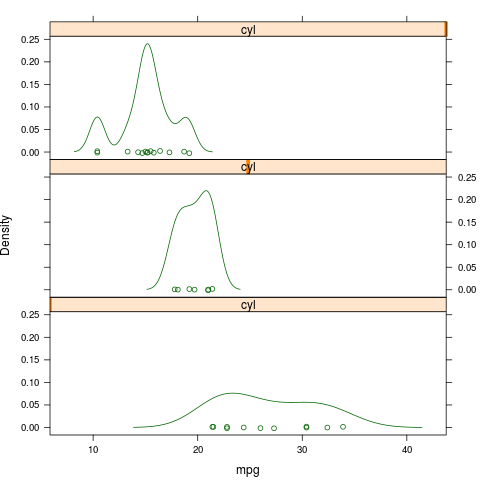
\includegraphics[width=0.6\columnwidth]{lattice-parameter2.png}
  \caption{在不同panel中绘制单变量分类数据}
\end{figure}
\end{onlyenv}

\begin{onlyenv}<3>
\begin{rcode}
> densityplot(~mpg, data=mtcars, |\colorbox{green}{group=cyl}|)
\end{rcode}
\begin{figure}
  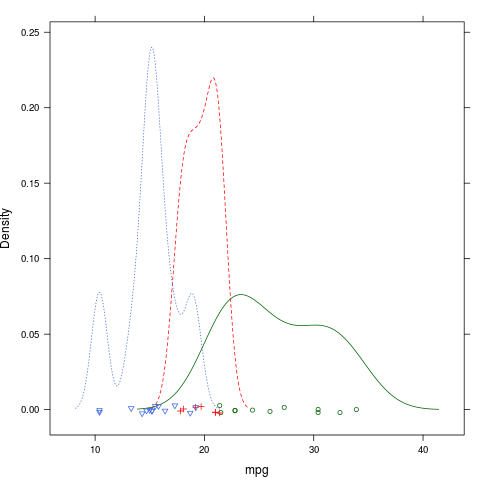
\includegraphics[width=0.6\columnwidth]{lattice-parameter3.png}
  \caption{在同一panel中绘制单变量分类数据}
\end{figure}
\end{onlyenv}

\begin{onlyenv}<4>
\begin{rcode}
> EE <- equal.count(ethanol$E, number=9, overlap=1/4)
> xyplot(|\colorbox{green}{NOx$\sim$ C \textbar EE}|, data = ethanol)
\end{rcode}
\begin{figure}
  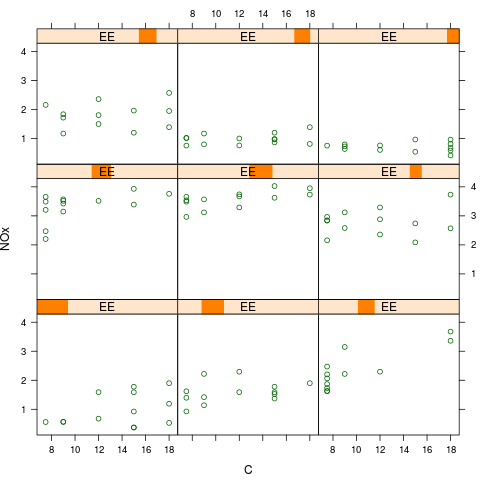
\includegraphics[width=0.6\columnwidth]{lattice-parameter4.png}
  \caption{在不同panel中绘制多变量分类数据}
\end{figure}
\end{onlyenv}
\end{frame} 

\begin{frame}[t]{\subsecname}{标准高级绘图函数}
\begin{itemize}
\item lattice包中提供了大量标准高级绘图函数用于直接绘制常用的统计图形
\end{itemize}
\vspace{-5pt}
\begin{figure}\centering
    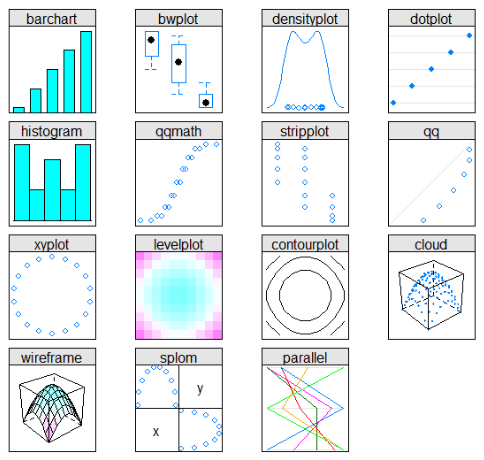
\includegraphics[width=0.6\columnwidth]{lattice-all.png}
    \caption{lattice中的标准高级绘图函数}
\end{figure}
\end{frame} 

\begin{frame}[t]{\subsecname}{标准高级绘图函数}
  \begin{table} \centering \scriptsize
    \begin{tabular}{|>{\centering\arraybackslash} m{0.2\columnwidth}|>{\centering\arraybackslash} m{0.2\columnwidth}|>{\centering\arraybackslash} m{0.2\columnwidth} |>{\centering\arraybackslash} m{0.2\columnwidth}|}
      \toprule
      \rowcolor{LightCyan}
      \multicolumn{1}{|c|}{\textbf{lattcie函数}} & \multicolumn{1}{c|}{\textbf{公式参数}} &
\multicolumn{1}{c|}{\textbf{描述}} & \multicolumn{1}{c|}{\textbf{graphics对应函数}} \\\hline
      barchart() & $y\sim x$ & 条形图 & barplot() \\\hline
      bwplot() & $y\sim x$ & 箱线图 & boxplot() \\\hline
      densityplot() & $\sim y$ & 核密度图 & plot.density()\\\hline
      dotplot() & $\sim y$ & Cleveland点图 & dotchart()\\\hline
      histogram() & $\sim x$ & 直方图 & hist()\\\hline
      stripplot() & $\sim y$ & 带状图 & stripchart()\\\hline
      xyplot() & $y\sim x$ & 散点图 & plot()\\\hline
      contourplot() & $z\sim x*y$ & 等高线图 & contour()\\\hline
      cloud() & $z\sim x*y$ &三维散点图 & 无\\\hline
      levelplot() & $z\sim x*y$ & 颜色图 & image()\\\hline
      wireframe() & $z\sim x*y$ & 三维透视图 & persp()\\\hline
      qq() & $\sim x$ & QQ图 & qqnorm()\\\hline
      splom() & $\sim data.frame$ & 散点图矩阵 & pairs()\\\hline
      parallel() & $\sim data.frame$ & 平行坐标图 & 无 \\
      \bottomrule
    \end{tabular}
    \caption{lattice包与graphics包的对应函数}
  \end{table}
\end{frame} 

\begin{frame}[t,fragile]{\subsecname}{panel函数和strip函数}
\begin{itemize}
\item lattice中每个高级绘图函数都有默认的panel参数和strip参数,
实质上对应的是两个匿名函数:\emphText{panel()和strip()}
\item 这两个函数可以用来对panel区域和strip区域需要绘制图形以及显示的
分类描述信息进行自定义扩展
%\item lattice也可以通过\emphText{update()}函数修改既有trellis对象中的绘图要素,从而达到修改图形的目的
\end{itemize}
\end{frame} 

\begin{frame}[c,fragile]{\subsecname}{panel函数和strip函数}
\begin{onlyenv}<1>
\begin{rcode}
# 在高级绘图函数中自定义panel和strip的示例
types.plain <- c("p", "l", "o", "r", "g", "s", "S", "h", "a", "smooth")
types.horiz <- c("s", "S", "h", "a", "smooth")
horiz <- rep(c(FALSE, TRUE), c(length(types.plain), length(types.horiz)))
types <- c(types.plain, types.horiz)
x <- sample(seq(-10, 10, length.out = 15), 30, TRUE)
y <- x + 0.25 * (x + 1)^2 + rnorm(length(x), sd = 5)

xyplot(y ~ x |\textbar| gl(1, length(types)),
       xlab = "type", 
       ylab = list(c("horizontal=TRUE", "horizontal=FALSE"), y = c(1/6, 4/6)), as.table = TRUE, layout = c(5, 3), between = list(y = c(0, 1)),
       # 自定义strip函数,...参数表示直接继承xyplot中的其他参数       
       |\colorbox{green}{strip = function(...)}|{
           # 调用标准panel函数panel.fill填充每个strip的颜色
           |\colorbox{green}{panel.fill}|(trellis.par.get("strip.background")$col[1])
           type <- types[panel.number()]
           # 调用底层grid绘图函数
           grid::grid.text(label = sprintf('"%s"', type), x = 0.5, y = 0.5)
           grid::grid.rect()
       },
       scales = list(alternating = c(0, 2), tck = c(0, 0.7), draw = FALSE),
       par.settings = list(layout.widths = list(strip.left = c(1, 0, 0, 0, 0))),
       # 自定义panel函数,...参数表示直接继承xyplot中的其他参数       
       |\colorbox{green}{panel = function(...)}| {
           type <- types[panel.number()]
           horizontal <- horiz[panel.number()]
           # 调用标准panel函数panel.xyplot按照预设参数每个panel中绘制图形  
           |\colorbox{green}{panel.xyplot}|(..., 
                        type = type,
                        horizontal = horizontal)
       })[rep(1, length(types))]
\end{rcode}
\end{onlyenv}

\begin{onlyenv}<2>
\begin{figure}\centering
    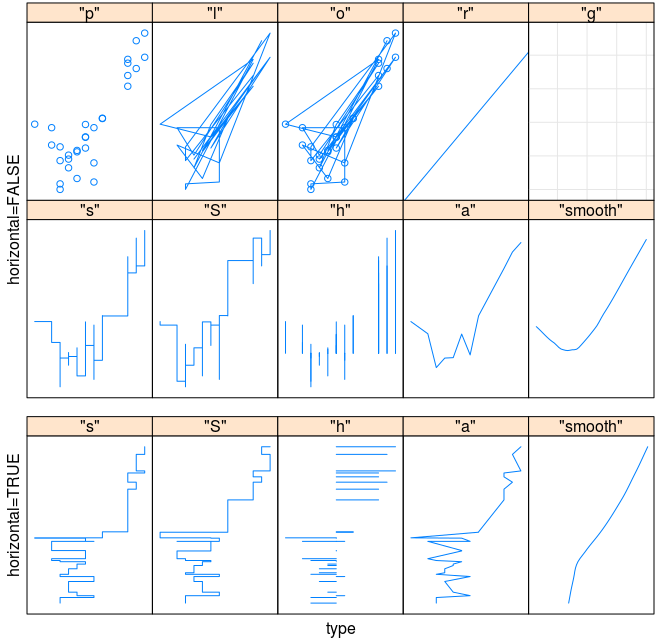
\includegraphics[width=0.7\columnwidth]{panel-example1.png}
    \caption{在高级绘图函数xyplot中自定义panel和strip}
\end{figure}
\end{onlyenv} 
\end{frame}

\begin{frame}[c,fragile]{\subsecname}{panel函数和strip函数}
\begin{figure}
 \begin{columns}
    \begin{column}[c]{.45\textwidth}
        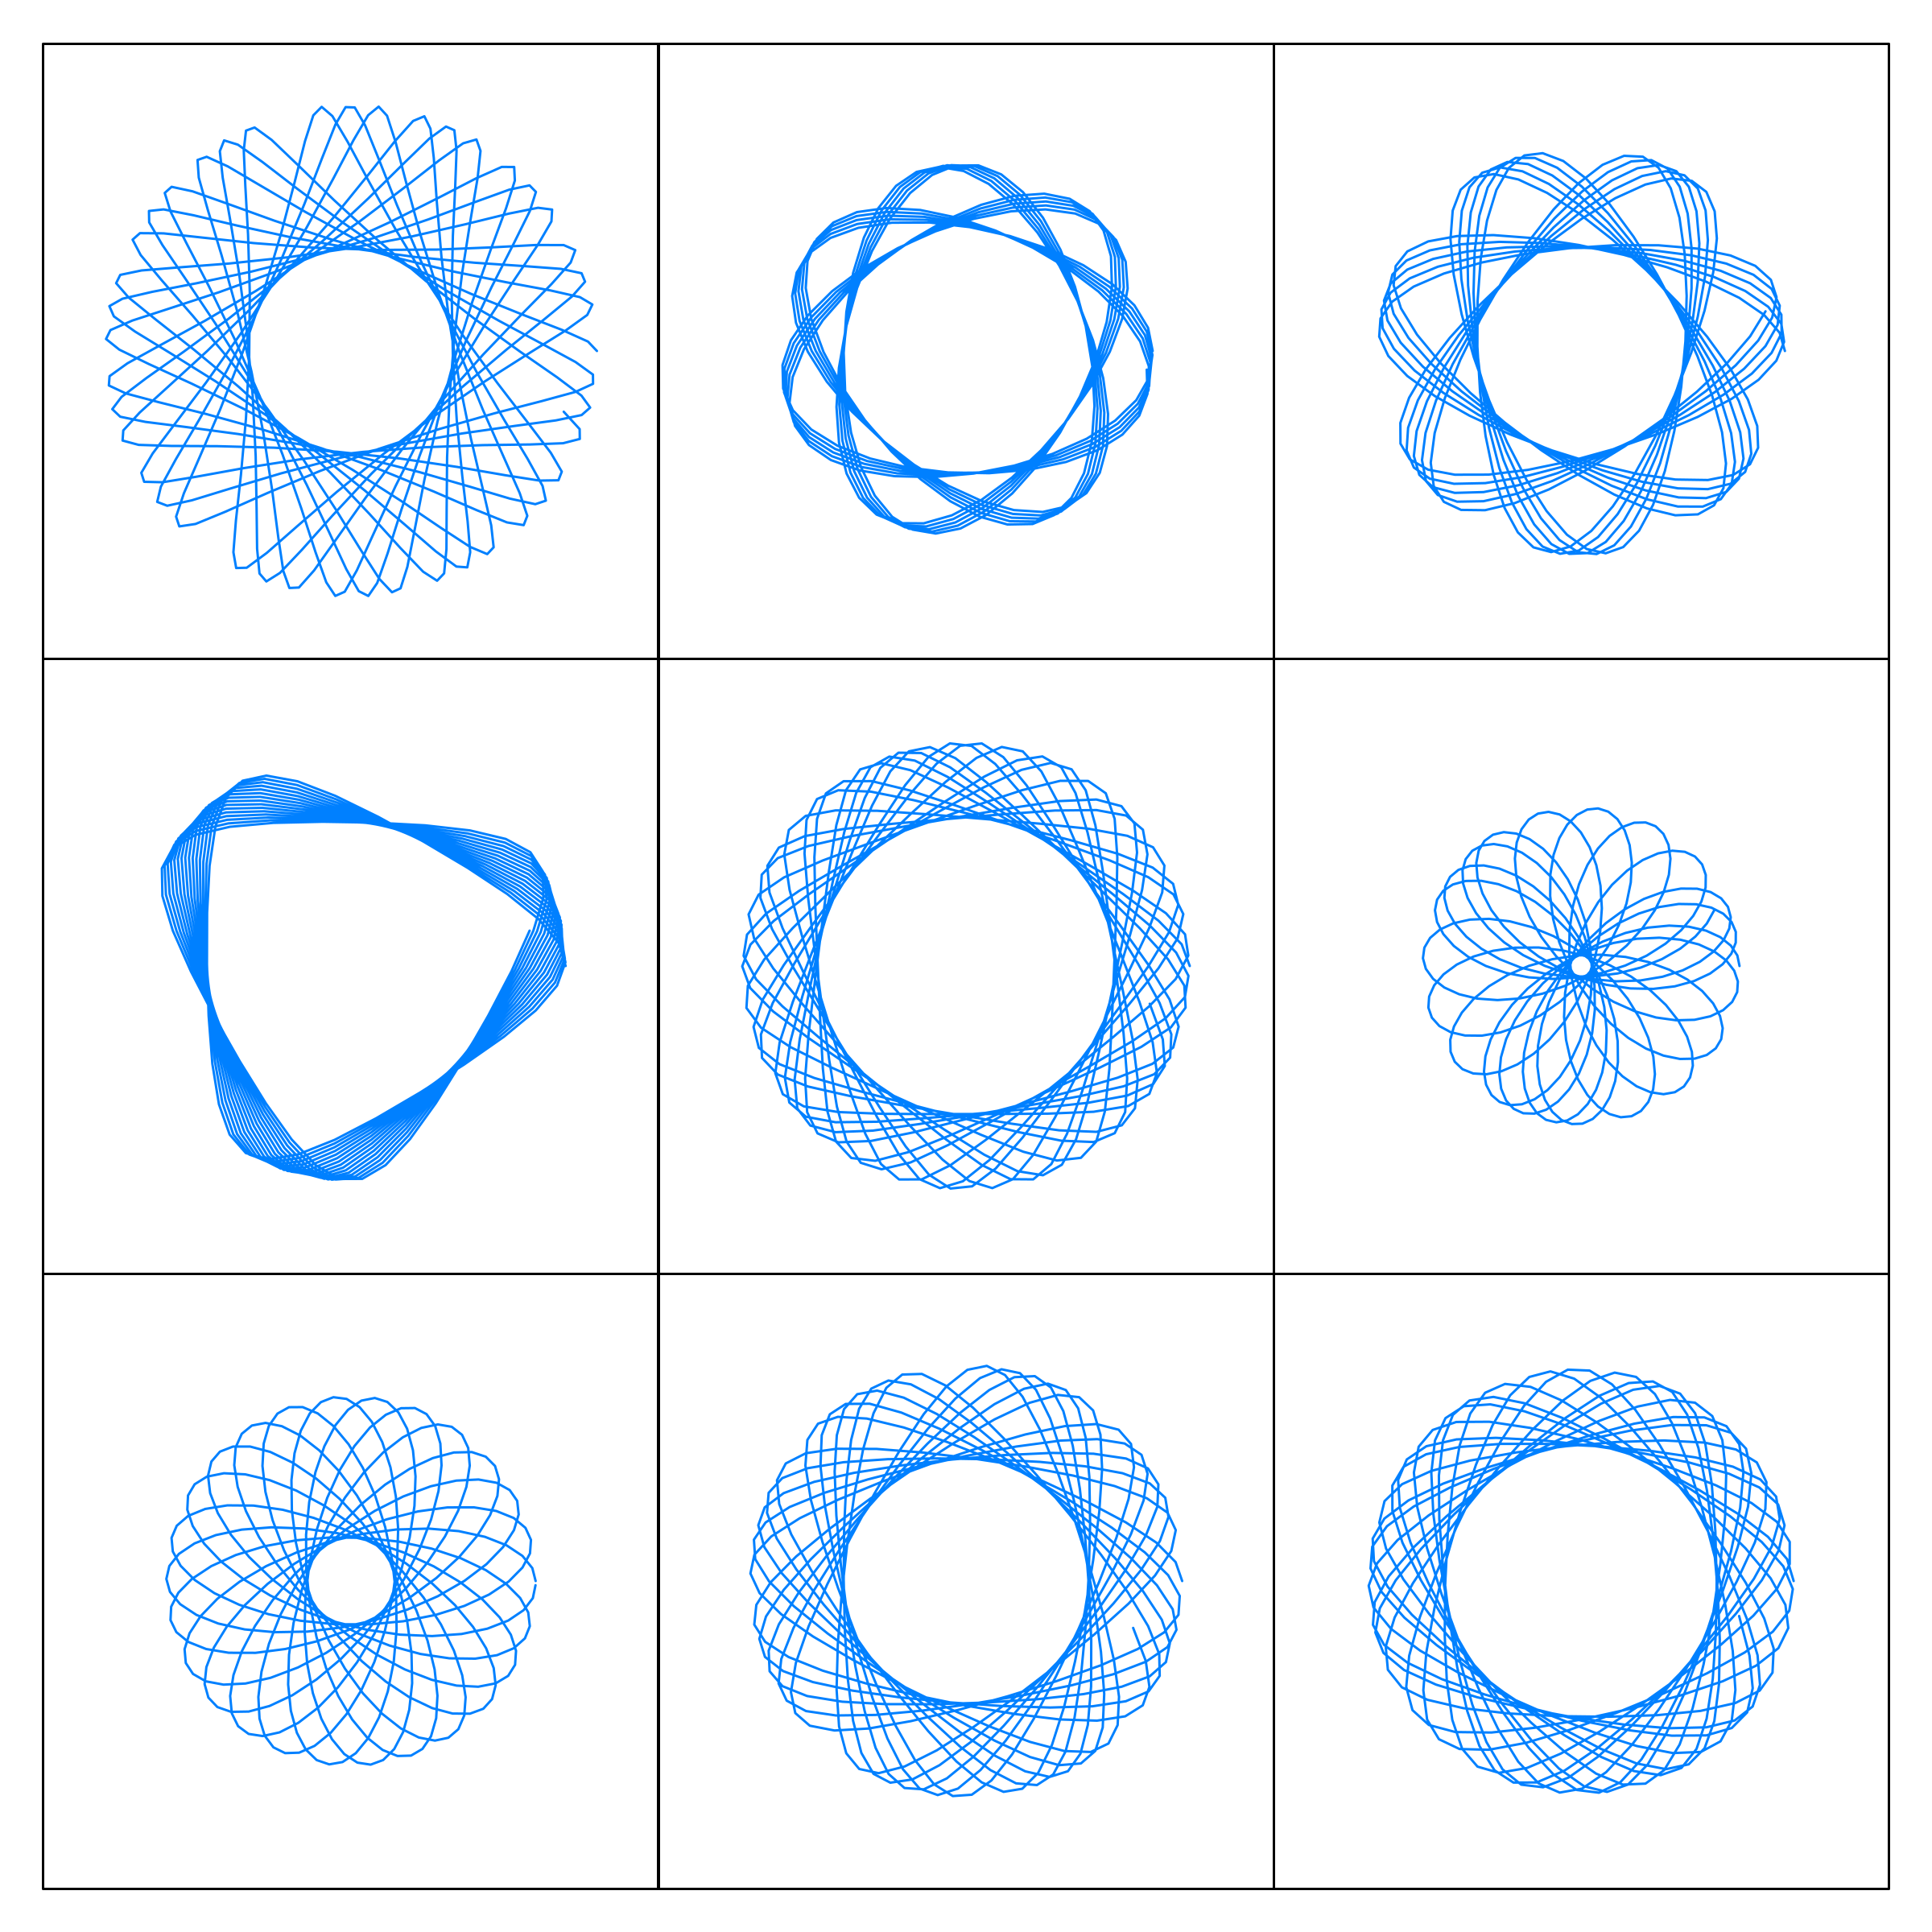
\includegraphics[width=\columnwidth]{panel-example2.png}
    \end{column}

    \begin{column}[c]{.55\textwidth}
\begin{rcode}
# 自定义一个panel函数绘制内旋轮线
# 注意:这个函数的所有参数都不是必选参数,而且没有...参数,这意味外部数据无法传入该函数参与绘图
> panel.hypotrochoid <- function(r, d, cycles = 10, density = 30)
 {
     if (missing(r)) r <- runif(1, 0.25, 0.75)
     if (missing(d)) d <- runif(1, 0.25 * r, r)
     t <- 2*pi*seq(0,cycles,by = 1/density)
     x <- (1-r)*cos(t)+d*cos((1-r)*t/r)
     y <- (1-r)*sin(t)-d*sin((1-r)*t/r)
     panel.lines(x, y)
 }
# 自定义prepanel函数来绘制panel的外框
> prepanel.hypocycloid <- function(x, y) {
     list(xlim=c(-1, 1),ylim = c(-1, 1))
 }

# 将xyplot函数传递给一个trellis对象p,这里传入的x参数其实并没有参与绘图
> p <- xyplot(x=c(-1, 1) ~ c(-1, 1), aspect = 1, cycles = 15, scales = list(draw = FALSE), xlab = "", ylab = "", panel = |\colorbox{green}{panel.hypotrochoid}|)
# 对象p循环绘图
> p[rep(1, 9)]
\end{rcode}
    \end{column}
  \end{columns}
  \caption{通过外部自定义panel函数来绘制图形}
\end{figure}
\end{frame} 

\begin{frame}[t,fragile]{\subsecname}{主题和图形参数设置}
\begin{itemize}
\item 在lattice中,所有的trellis对象都有一个主题(theme),theme中包含完整的图形要素:颜色、线宽、字体等
\item 当前theme的参数可以直接通过\emphText{trellis.par.get()}函数获取,通过
\emphText{trellis.par.set()}函数直接修改;\emphText{对theme参数的设置作用于当前绘图设备中的
所有高级绘图函数}
\end{itemize}
%\vspace{-10pt}

\begin{overlayarea}{\textwidth}{\textheight}
\begin{onlyenv}<1>
\begin{rcode}
# 罗列trellis对象中的所有图形参数
> names(trellis.par.get())
 [1] "grid.pars"         "fontsize"          "background"       
 [4] "panel.background"  "clip"              "add.line"         
 [7] "add.text"          "plot.polygon"      "box.dot"          
[10] "box.rectangle"     "box.umbrella"      "dot.line"         
[13] "dot.symbol"        "plot.line"         "plot.symbol"      
[16] "reference.line"    "strip.background"  "strip.shingle"    
[19] "strip.border"      "superpose.line"    "superpose.symbol" 
[22] "superpose.polygon" "regions"           "shade.colors"     
[25] "axis.line"         "axis.text"         "axis.components"  
[28] "layout.heights"    "layout.widths"     "box.3d"           
[31] "par.xlab.text"     "par.ylab.text"     "par.zlab.text"    
[34] "par.main.text"     "par.sub.text"    
\end{rcode}
\end{onlyenv}

\vspace{-10pt}
\begin{onlyenv}<2>
\begin{figure}[ht]
  \centering
  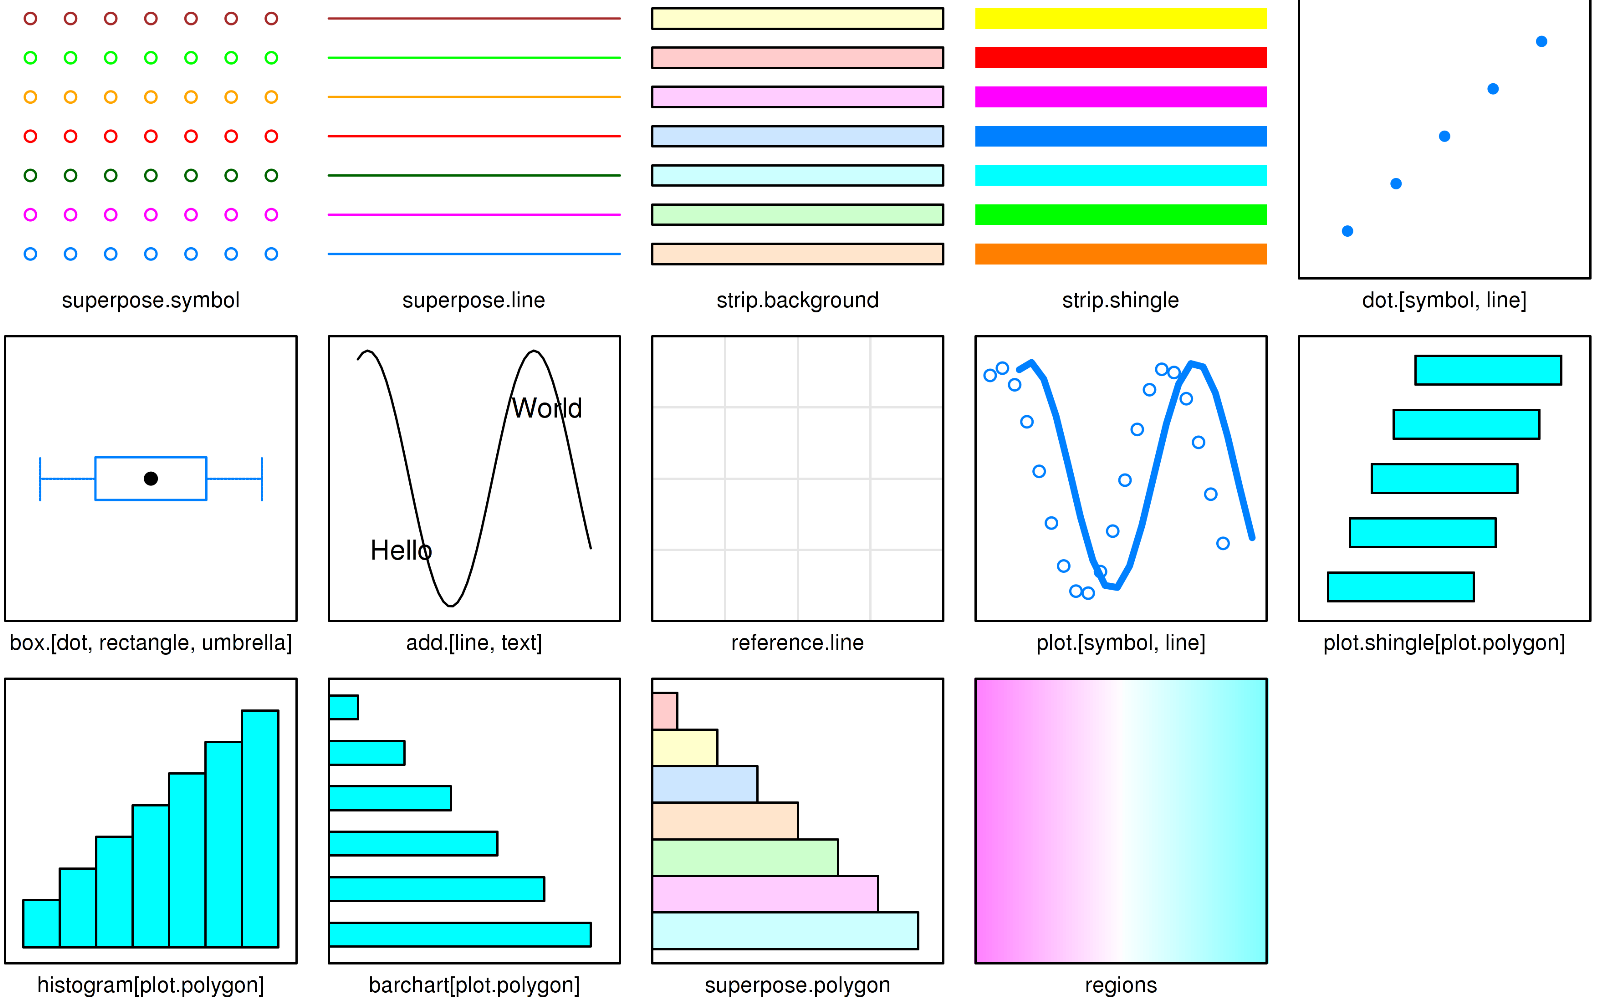
\includegraphics[width=0.7\columnwidth]{show_settings.png}
  \caption{trellis对象中所有的图形参数}
\end{figure}
\end{onlyenv}

\begin{onlyenv}<3>
\begin{figure}
 \begin{columns}
    \begin{column}[c]{.4\textwidth}
        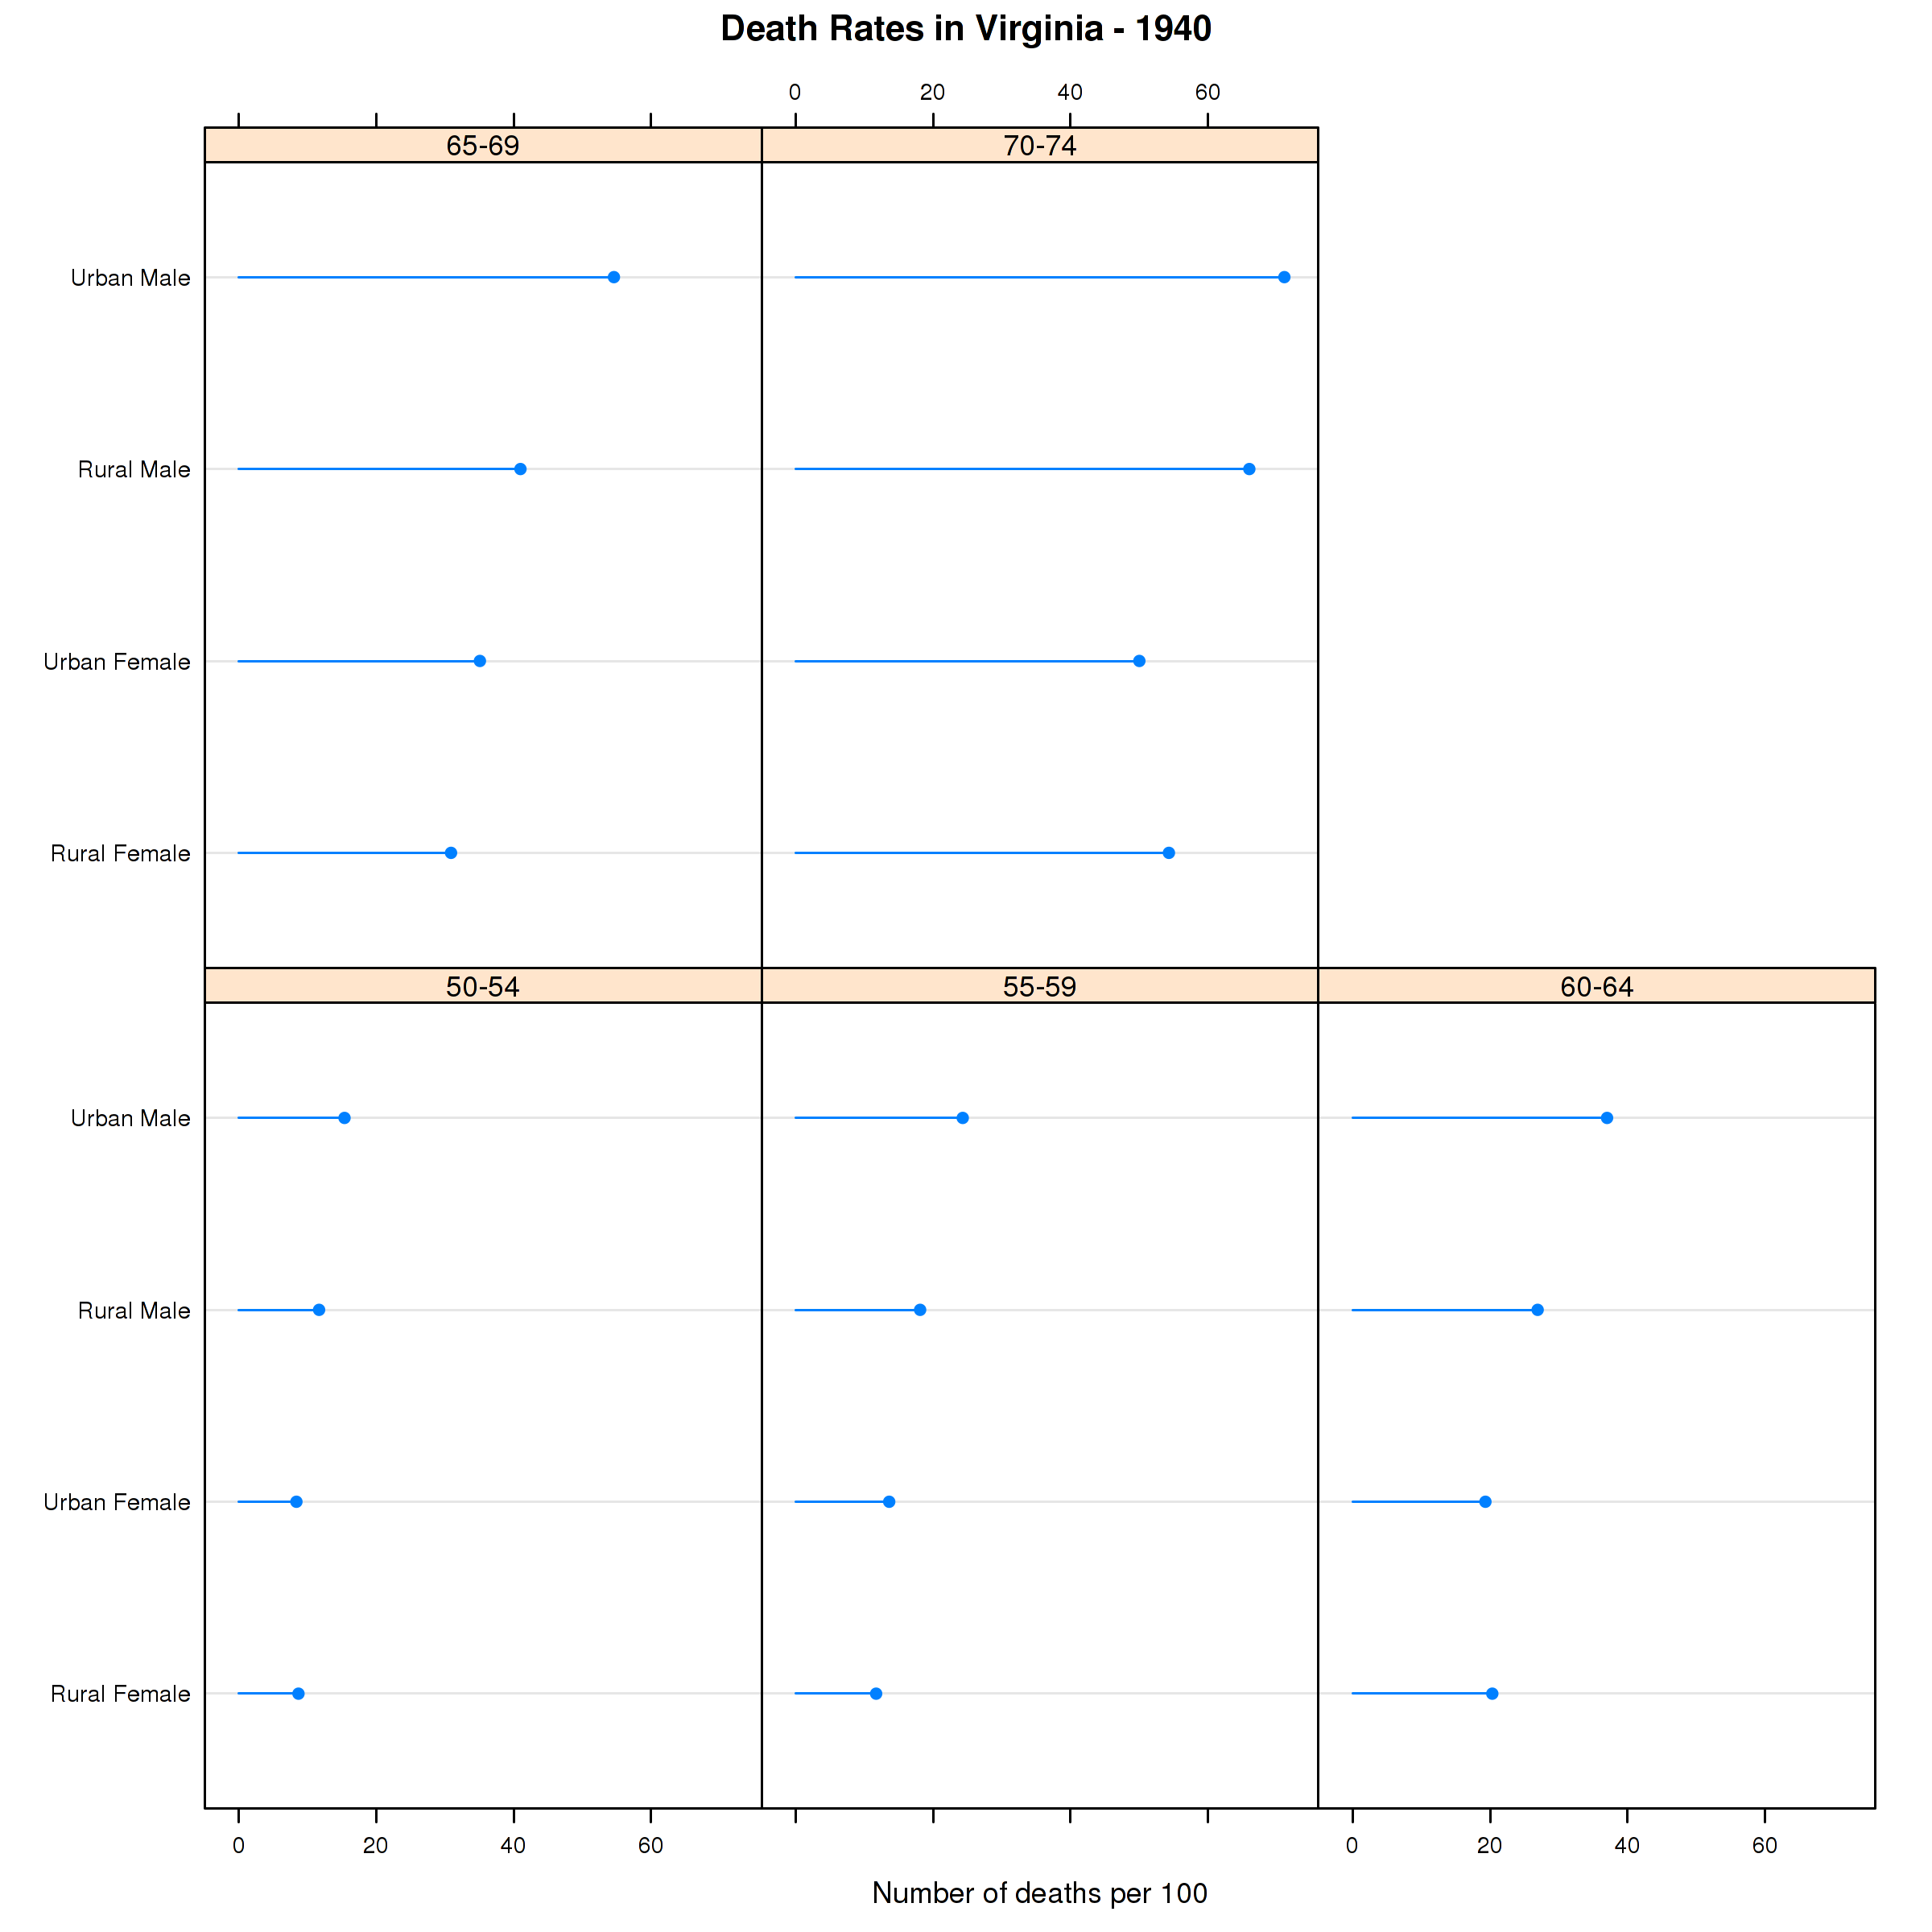
\includegraphics[width=\columnwidth]{trellis_par_set1.png}
    \end{column}

    \begin{column}[c]{.6\textwidth}
\begin{rcode}
# 绘制dotplot传递给trellis对象vad.plot
> vad.plot <- 
    dotplot(reorder(Var2, Freq)~Freq |\textbar| Var1,
            data = as.data.frame.table(VADeaths), 
            origin = 0, type = c("p", "h"),
            main = "Death Rates in Virginia - 1940", 
            xlab = "Number of deaths per 100")
> vad.plot
\end{rcode}
    \end{column}
  \end{columns}
  \caption{通过直接修改trellis对象的图形参数实现修改图形}
\end{figure}
\end{onlyenv}

%\vspace{-10pt}
\begin{onlyenv}<4>
\begin{figure}
 \begin{columns}
    \begin{column}[c]{.4\textwidth}
        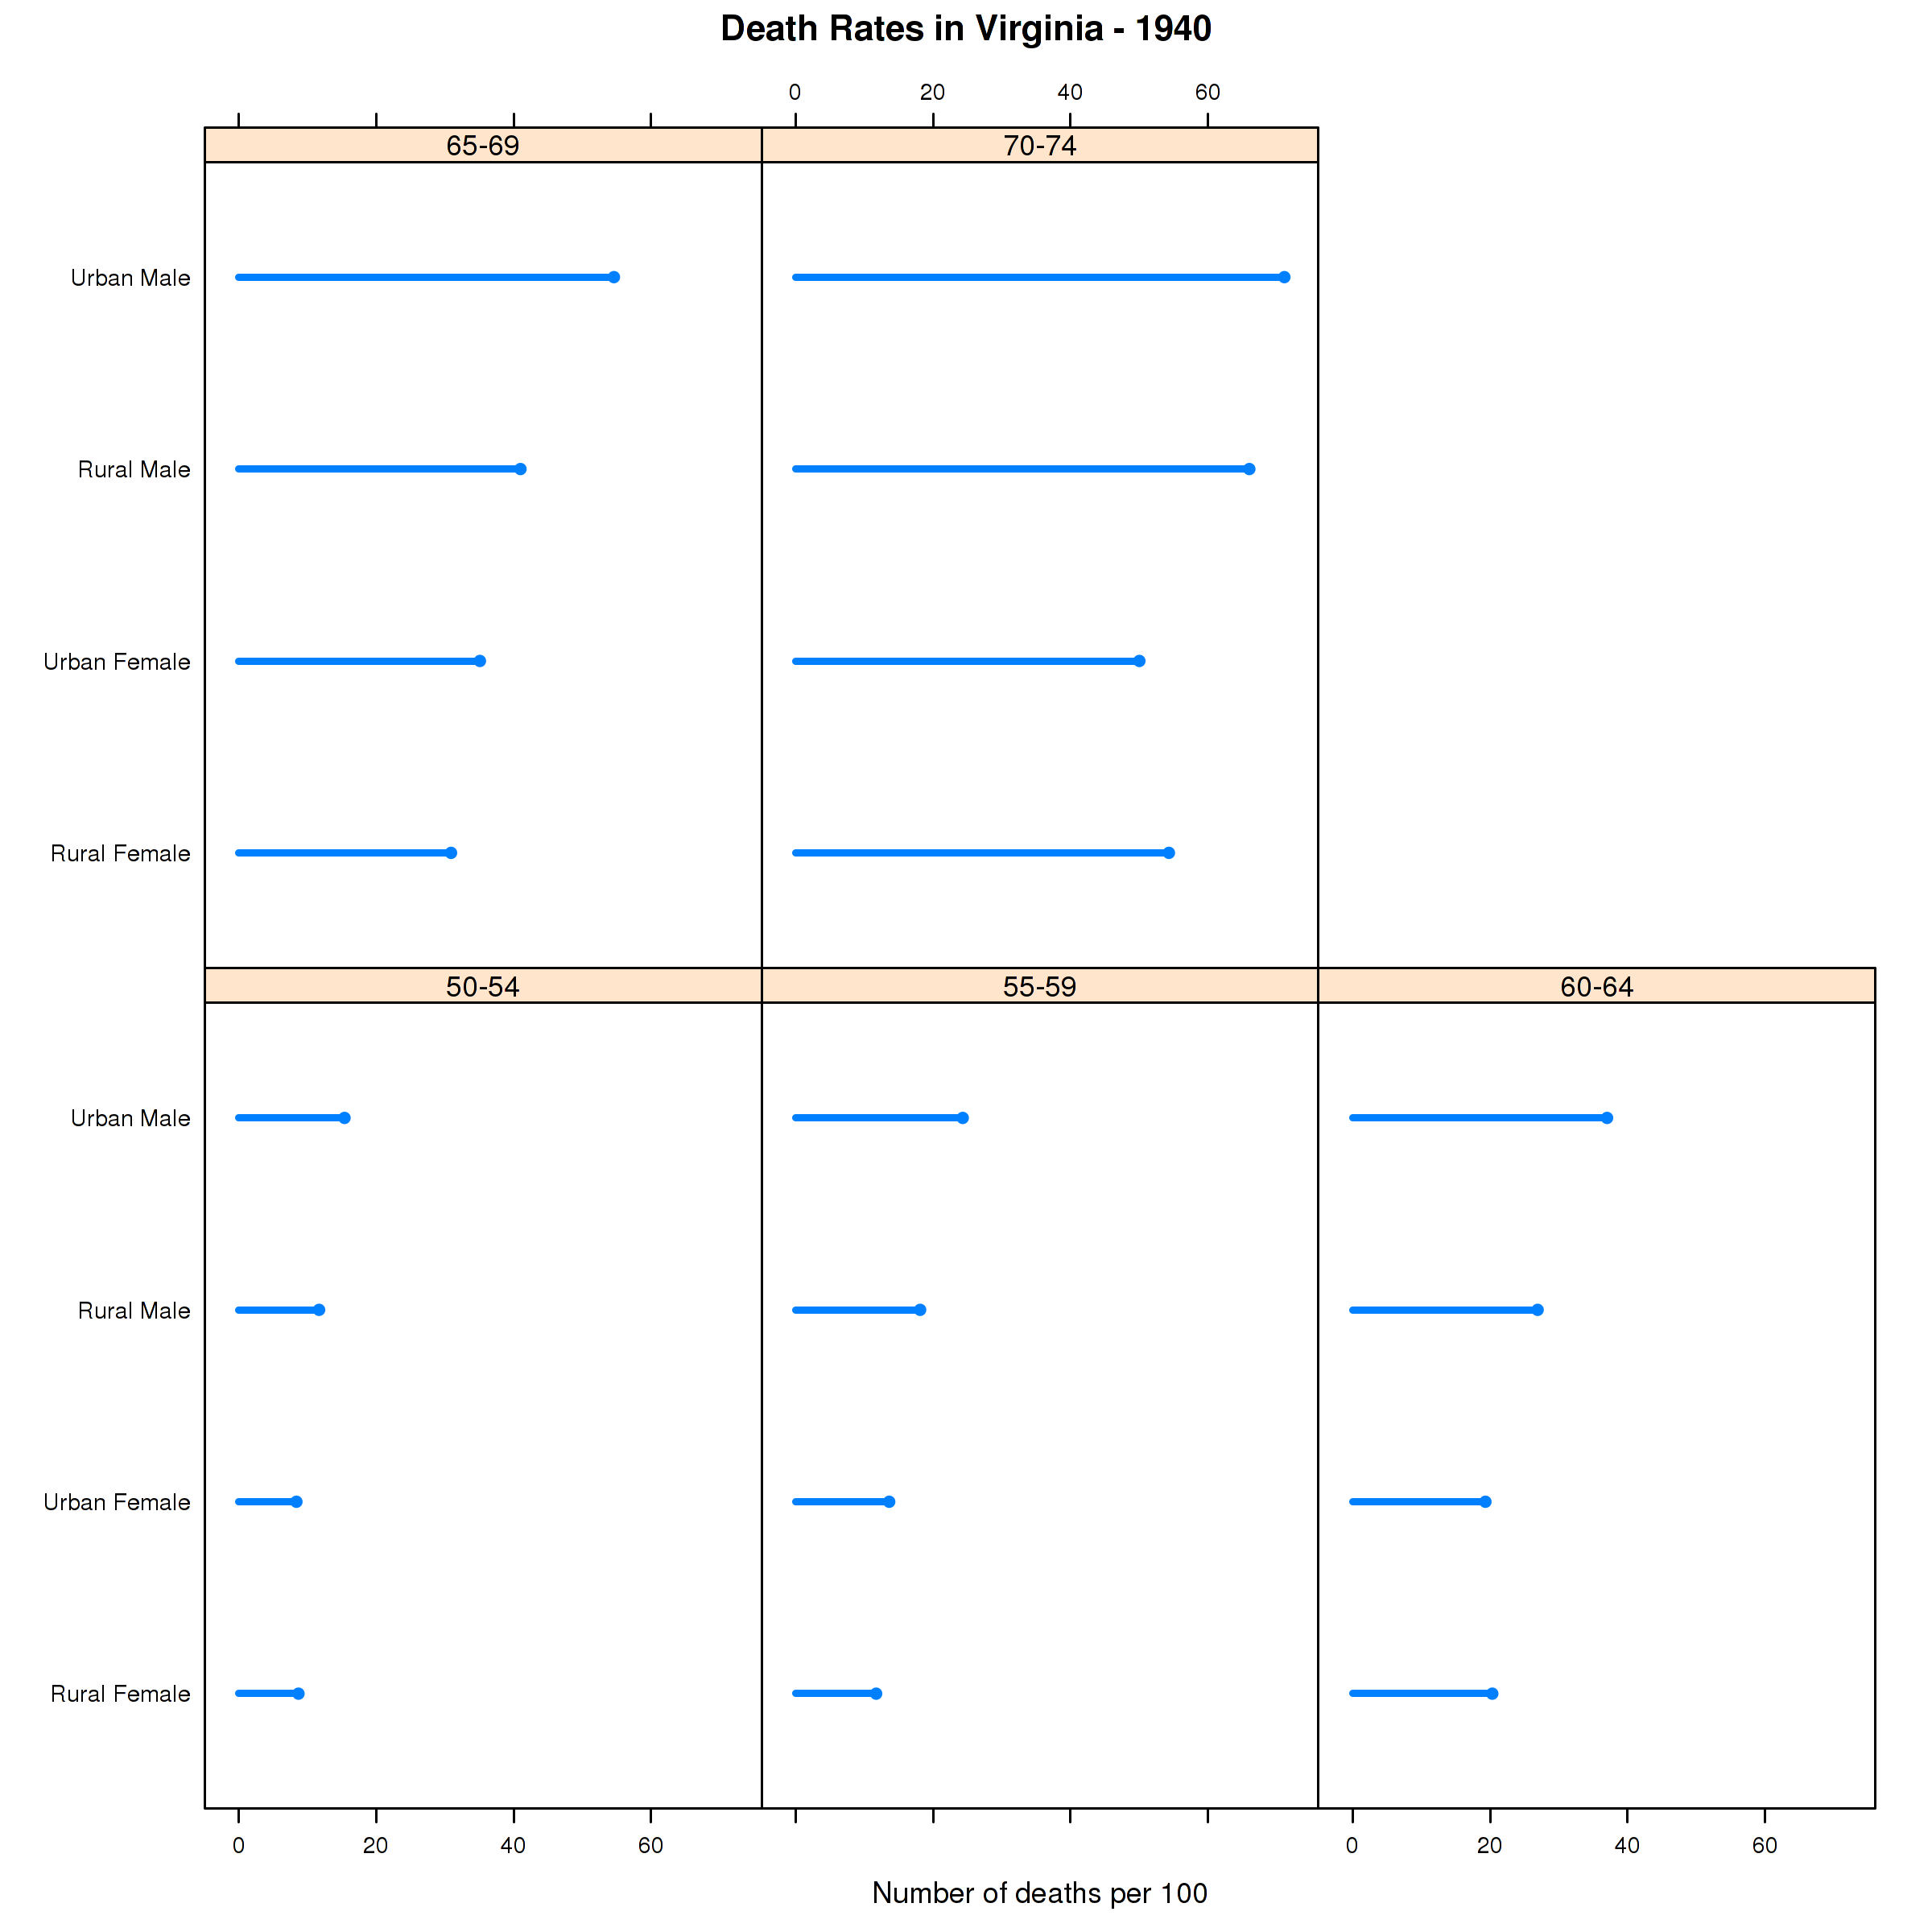
\includegraphics[width=\columnwidth]{trellis_par_set2.png}
    \end{column}

    \begin{column}[c]{.6\textwidth}
\begin{rcode}
# 在上图基础上修改绘图参数
# 获得当前主题的dot.line设置
> dot.line.settings <- |\colorbox{green}{trellis.par.get}|("dot.line")
# 将dot.line的颜色设置为透明不可见
> dot.line.settings$col <- "transparent"
# 应用新的参数设置
> |\colorbox{green}{trellis.par.set}|("dot.line", dot.line.settings)
# 获得当前主题的plot.line设置
> plot.line.settings <- |\colorbox{green}{trellis.par.get}|("plot.line")
# 将plot.line的线宽设置为3,默认是1
> plot.line.settings$lwd <- 3
# 应用新的参数设置
> |\colorbox{green}{trellis.par.set}|("plot.line", plot.line.settings)
> vad.plot
\end{rcode}
    \end{column}
  \end{columns}
  \caption{通过直接修改trellis对象的图形参数实现修改图形}
\end{figure}
\end{onlyenv}
\end{overlayarea}
\end{frame}

\begin{frame}[t,fragile]{\subsecname}{主题和图形参数设置}
\begin{itemize}
\item 除了设置theme参数之外,还可以通过\emphText{par.settings参数}仅对当前图形进行图形参数调整,
这比较类似par()函数的作用
\item 另外,lattice中提供了\emphText{update.trellis}函数来更新trellis对象的参数,
配合par.settings参数可以在不重绘图形的情况下实现图形的修改
\end{itemize}

\begin{overlayarea}{\textwidth}{\textheight}
\begin{onlyenv}<2>
\begin{figure}
 \begin{columns}
    \begin{column}[c]{.4\textwidth}
        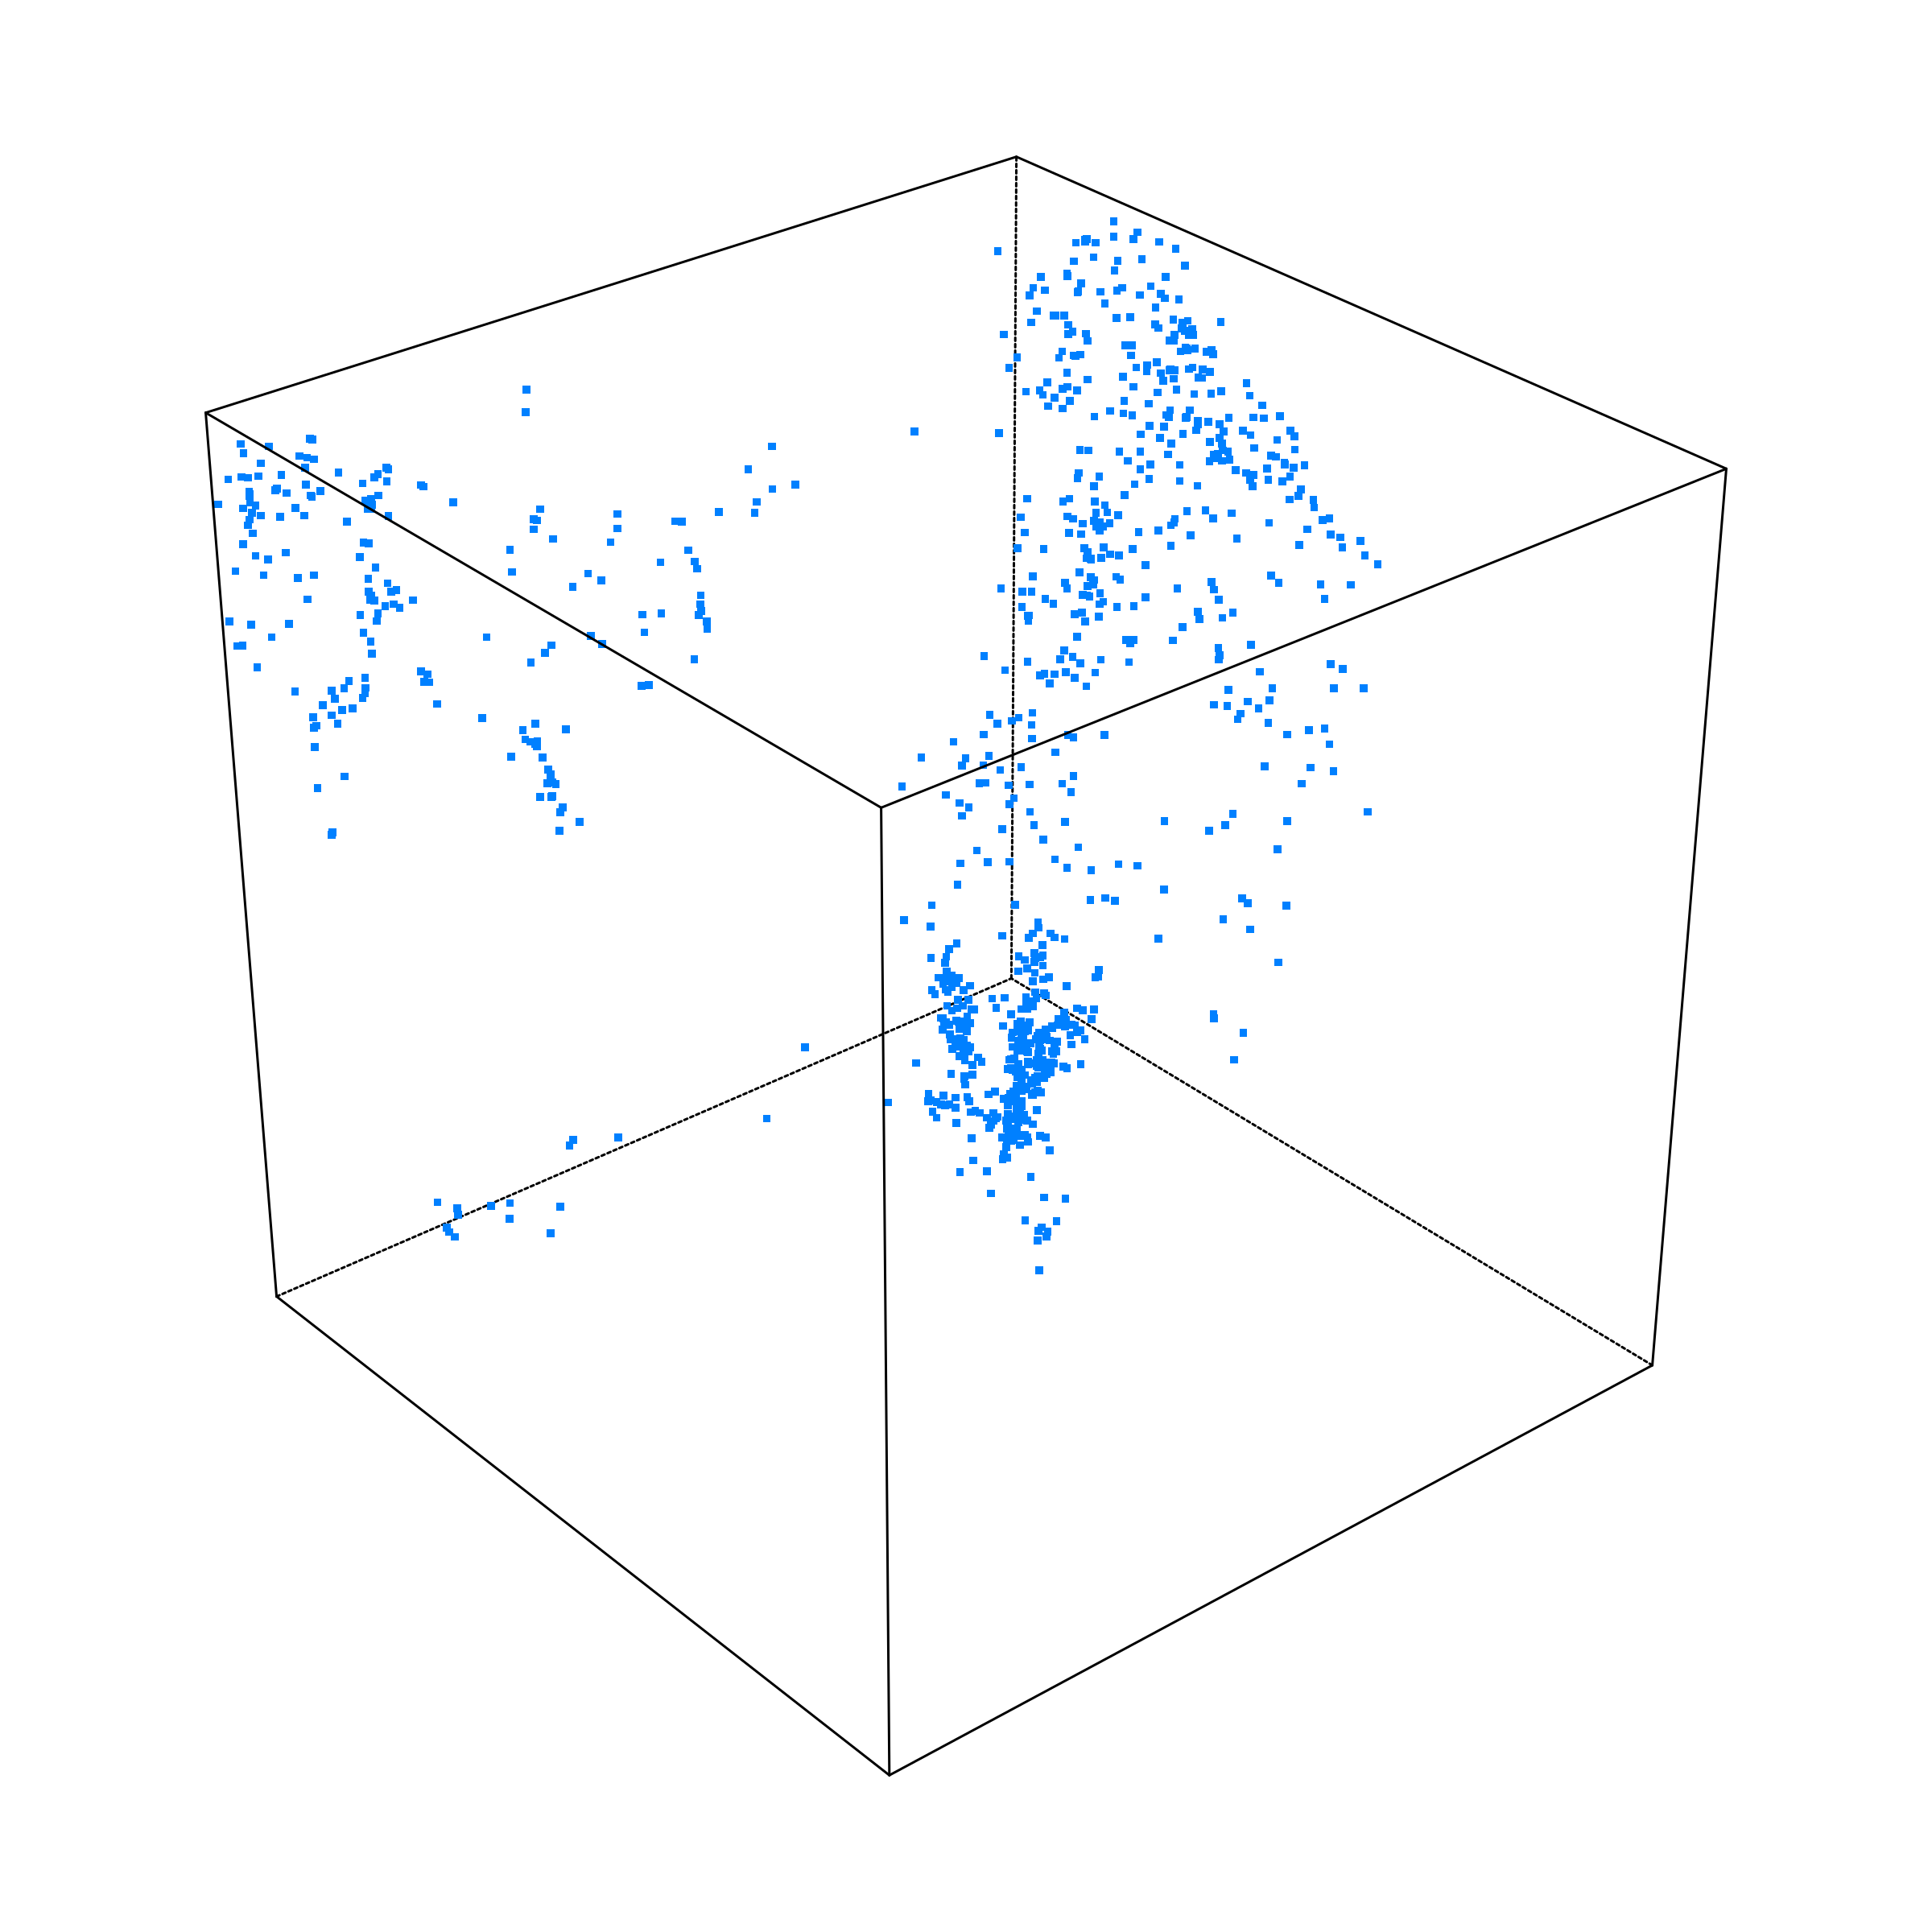
\includegraphics[width=\columnwidth]{update-example1.png}
    \end{column}

    \begin{column}[c]{.6\textwidth}
\begin{rcode}
# 首先定义一个三维散点图,并将其传入trellis对象p
> p <-
  cloud(depth ~ long + lat, quakes, zlim = c(690, 30), pch = ".", cex = 4, zoom = 1, xlab = NULL, ylab = NULL, zlab = NULL,scales = list(draw = FALSE),
        # 用par.settings参数设置坐标线为透明
        |\colorbox{green}{par.settings}|=list(axis.line = list(col = "transparent")))
> p
\end{rcode}
    \end{column}
  \end{columns}
  \caption{通过update函数和par.settings对象修改图形}
\end{figure}
\end{onlyenv}

\vspace{-10pt}
\begin{onlyenv}<3>
\begin{figure}
 \begin{columns}
    \begin{column}[c]{.4\textwidth}
        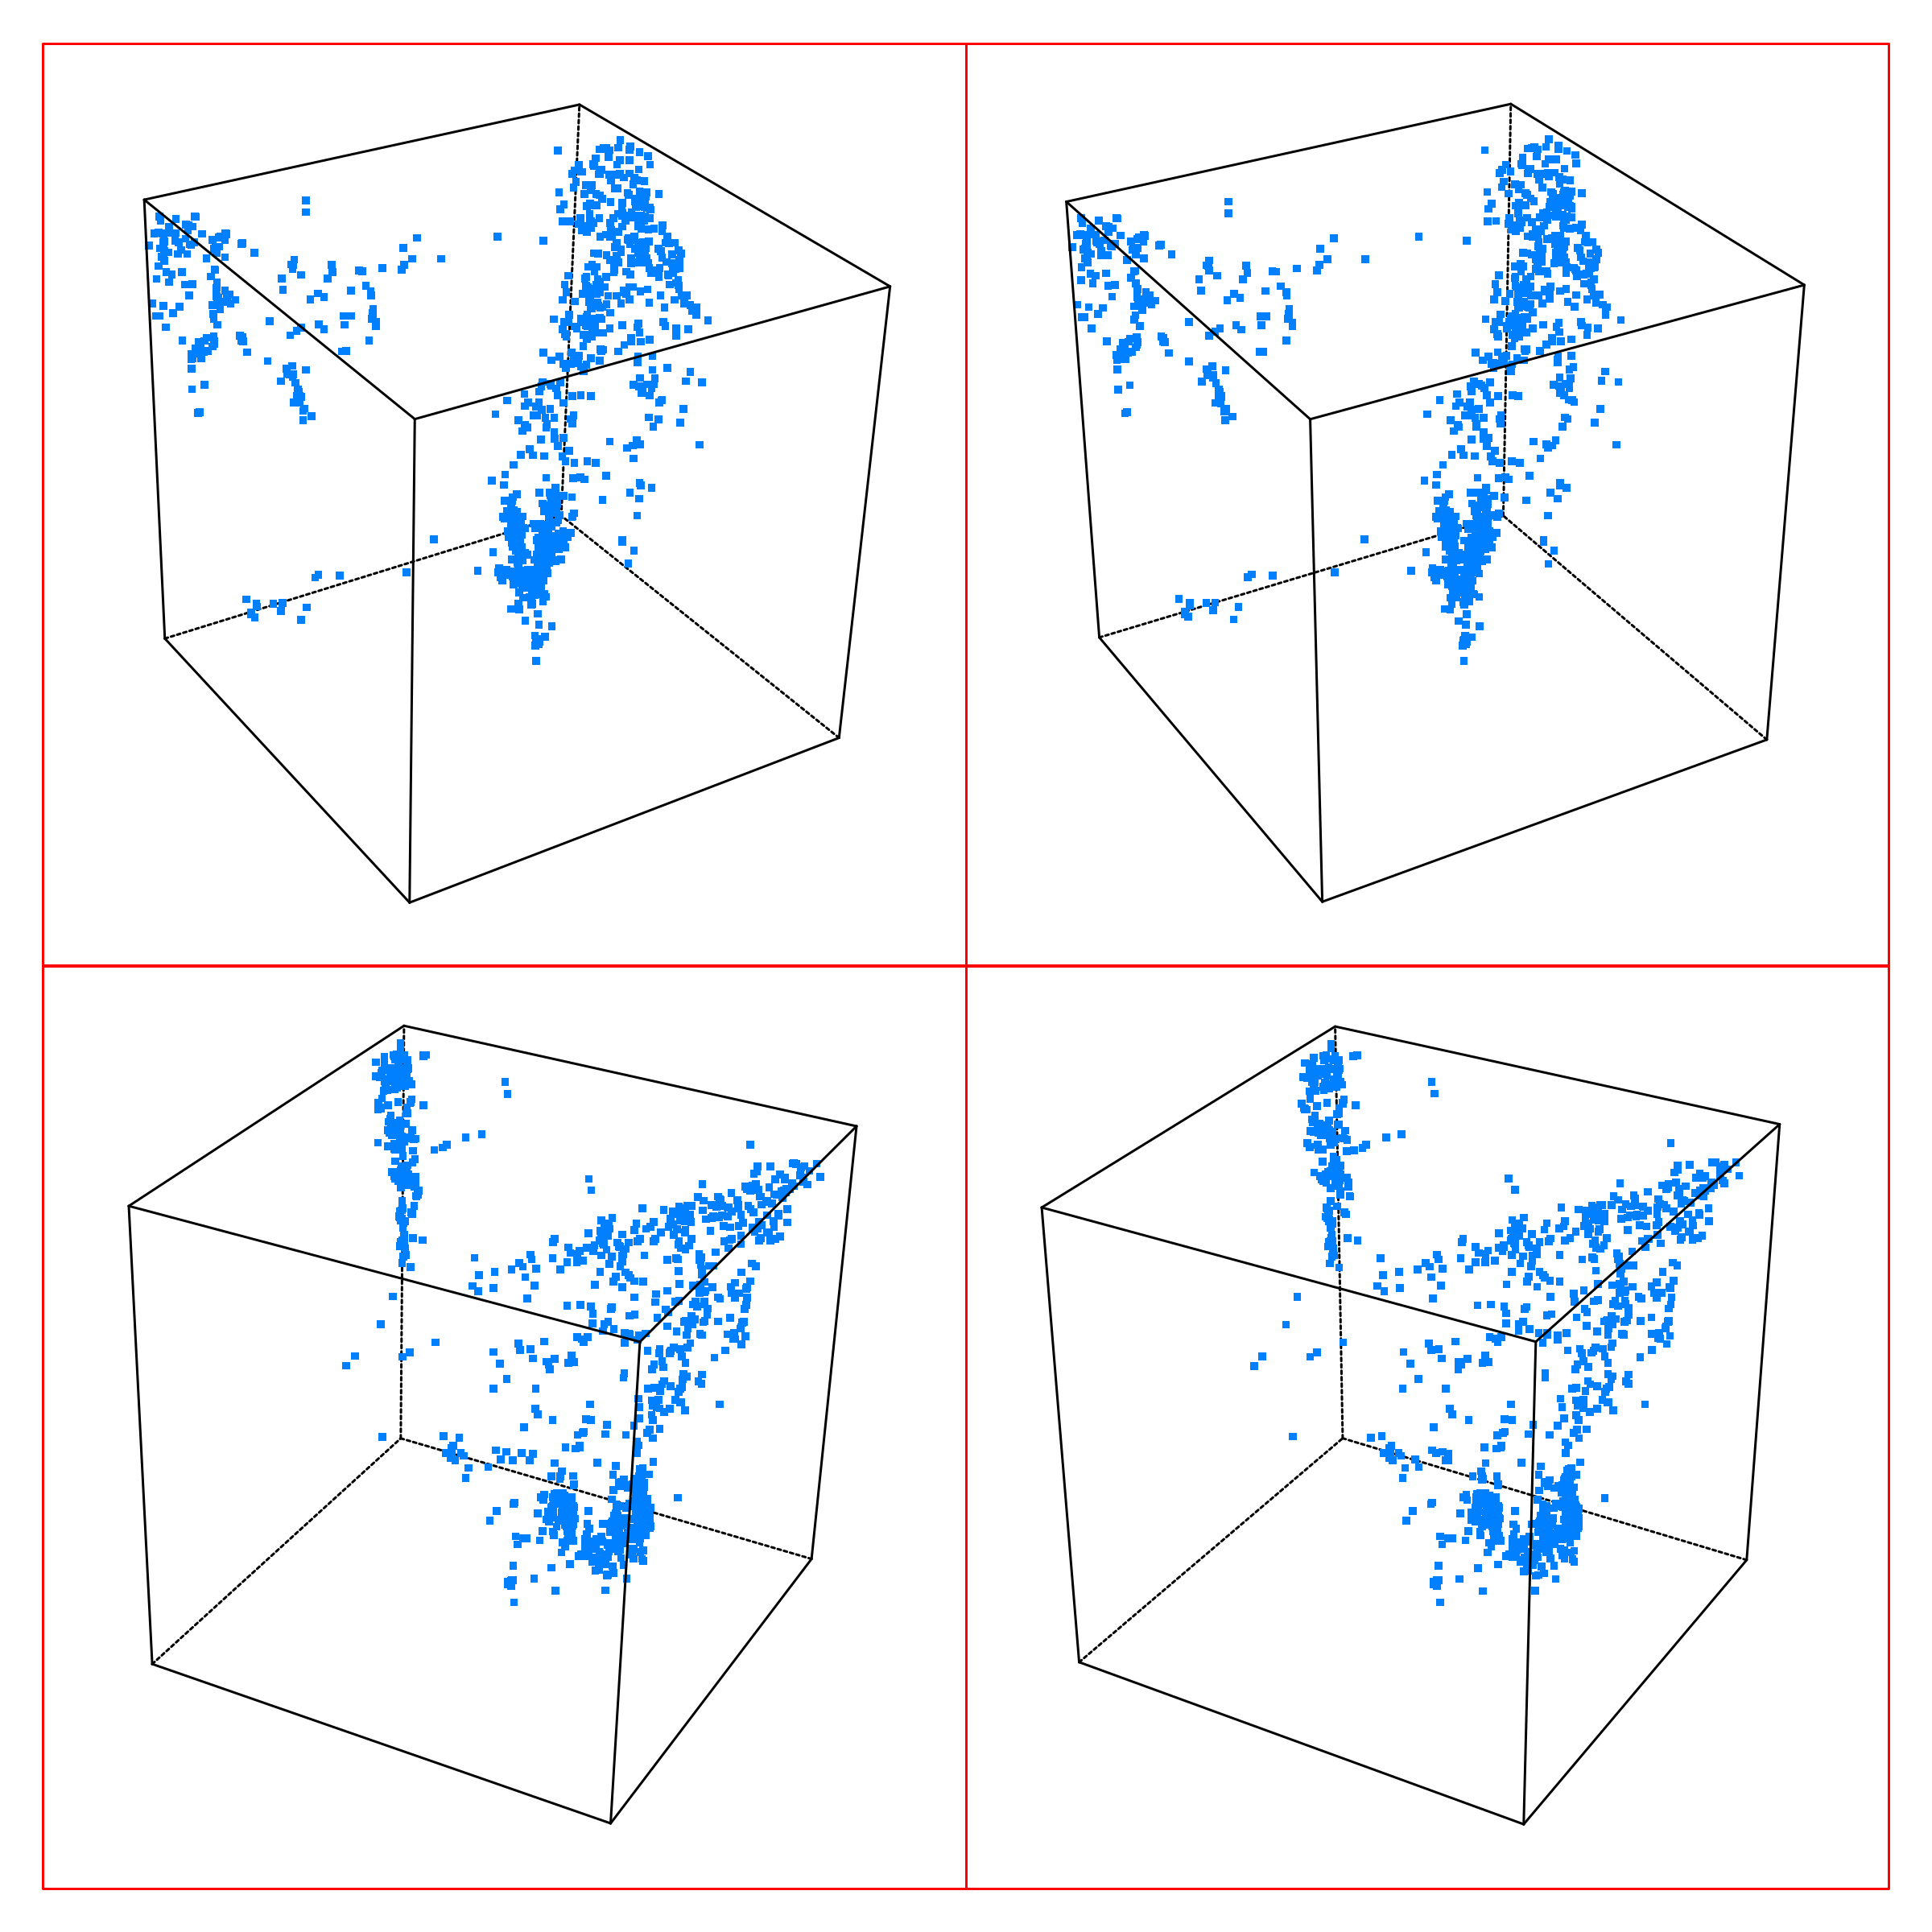
\includegraphics[width=\columnwidth]{update-example2.png}
    \end{column}

    \begin{column}[c]{.6\textwidth}
\begin{rcode}
> npanel <- 2
# 设置三维散点图的旋转视角
> rotz <- seq(-30, 30, length = npanel)
> roty <- c(3, 0)
# 用update.trellis函数更改原有图形
# 注意:由于update.trellis函数是一个继承自update函数的S3型对象,而传入的p是trellis对象,因此这里直接可以写update
> |\colorbox{green}{update}|(p[rep(1, 2 * npanel)], 
         layout = c(2, npanel),
         panel = function(..., screen) {
           crow <- current.row()
           ccol <- current.column()
         panel.cloud(..., screen = list(z = rotz[crow], x = -60, y = roty[ccol]))},
         # 用par.settings参数设置坐标线颜色为红 
         |\colorbox{green}{par.settings}|=list(axis.line=list(col="red")))
\end{rcode}
    \end{column}
  \end{columns}
  \caption{通过trellis对象的图形参数实现修改图形}
\end{figure}
\end{onlyenv}
\end{overlayarea}
\end{frame}

%https://www.cnblogs.com/nxld/p/6059603.html

\subsection{ggplot2程序包}
\begin{frame}{\subsecname}{}
\begin{itemize}
\item<1-> ggplot2是grid绘图系统的另一个广泛使用的实现包,由\href{http://hadley.nz/}{\uline{Hadley Wickham}}开发维护,\emphText{目前该包尚未纳入base包,需要单独下载} 
\item<2-> ggplot2的设计理念来自Leland Wilkinson的\emphText{《The Grammar of Graphics》}一书,其吸取了书中提出的绘图理论和优雅的绘图语法:\emphText{将绘图与数据分离,数据相关绘图与数据无关绘图分离}
\end{itemize}

%\vspace{-5pt}
\begin{overlayarea}{\textwidth}{\textheight}
\only<1>{
\begin{figure}[ht]
  \centering
  
\includegraphics[width=0.8\columnwidth]{hadley_wickham.png}
  \caption{ggplot2程序包的作者Hadley Wickham,目前是RStudio公司首席科学家}
\end{figure}}

\only<2->{
\begin{figure}[ht]
  \centering
  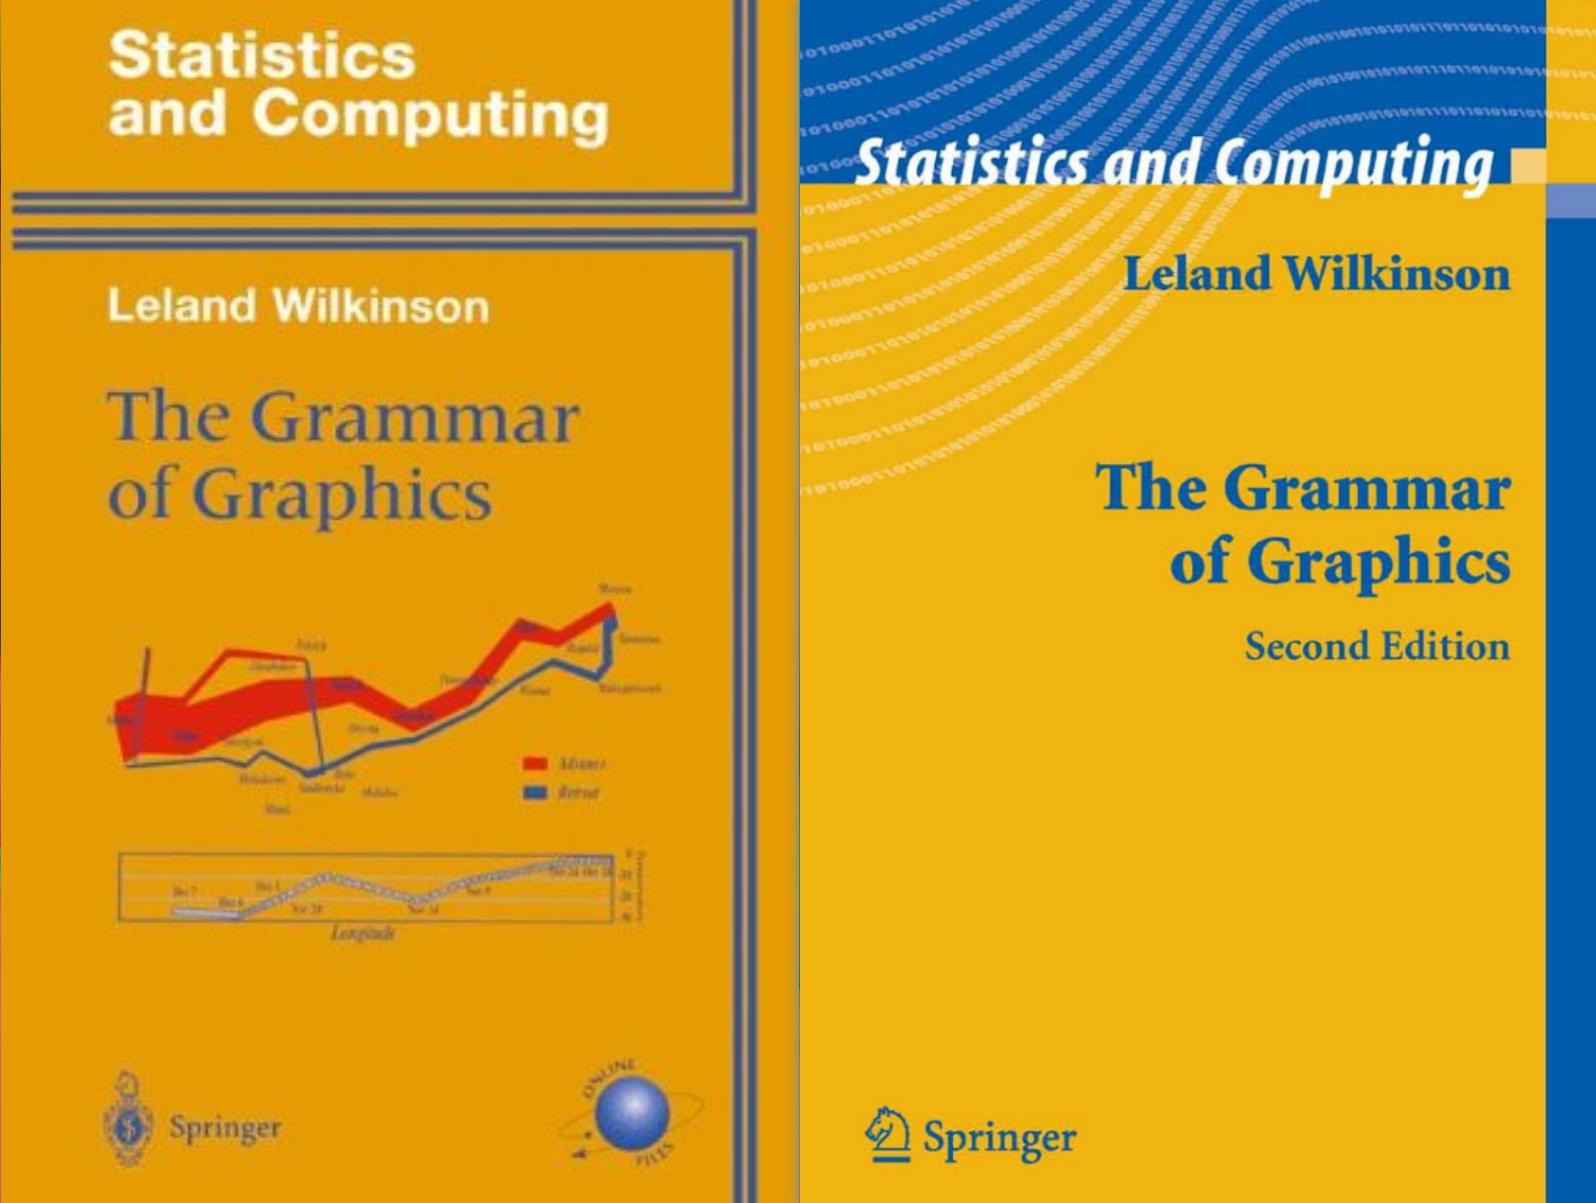
\includegraphics[width=0.55\columnwidth]{the_grammar_of_graphics.png}
  \caption{统计图形领域经典著作《The Grammar of Graphics》的第一版(1999)和第二版(2005),ggplot2的命名就取自这本书的首字母缩写再加上plot}
\end{figure}}

\end{overlayarea}
\end{frame}

